\documentclass[11pt,a4paper,english]{article}
\usepackage[titletoc, title]{appendix}
\usepackage{amsmath}
\usepackage{amssymb}
\usepackage{bm}
\usepackage{array}
\usepackage{babel}
\usepackage{bbding}
\usepackage{color}
\usepackage[normal]{caption}
\usepackage{subcaption}
\usepackage{epsfig}
\usepackage{graphicx}
\usepackage{pdflscape}
%\usepackage{multirow}
\usepackage{psfrag}
\usepackage{proofapnd}
\usepackage[round]{natbib}
%\usepackage{bbm}
%\usepackage[T1]{fontenc}
%\usepackage[normal]{caption2} % for caption
\usepackage{rotating}
\usepackage[margin=2cm]{geometry} % for the same margin
\usepackage{latexsym}
%\usepackage{subfig}
\usepackage{setspace}
\usepackage{slashbox}
\usepackage{enumitem}
\usepackage{booktabs}
\usepackage{tabularx}
\usepackage{longtable,booktabs}

\setlist[itemize]{leftmargin=*}
\setlist[description]{leftmargin=*}

%\setlength{\topmargin}{0.0 in} \setlength{\textwidth}{6in}
%\setlength{\oddsidemargin}{0.5in}
%\setlength{\evensidemargin}{-0.01in} \setlength{\textheight}{9in}
\captionsetup{font={onehalfspacing,small}, labelfont=bf}

\title{\LARGE \bf Hedging Futures with Spectral Risk Measures}
%\author{
%	\begin{tabular}[t]{ccc}
%		Lu, Meng-Jou\thanks{Corresponding author. 
%			Department of Information and Finance
%			Management, Institute of Finance and Institute of Information
%			Management, National Chiao-Tung University, No.1001 Daxue Rd,
%			Hsinchu City, Taiwan. Ladislaus von Bortkiewicz Chair of Statistics,
%			Humboldt--Universit\"{a}t zu Berlin, C.A.S.E. -- Center for
%			Applied Statistics and Economics, Unter den Linden 6, 10099 Berlin, Germany.
%     E-mail: \texttt{mangrou@gmail.com}.}
%		 \and\and Nguyen, Phuong Anh   
%		\thanks{Department of Finance and Banking, School of Business, International University-VNUHCM, Ho Chi Minh City, Vietnam. E-mail:
%			\texttt{npanh@hcmiu.edu.vn}. }
%			\and\and  H\"{a}rdle, Wolfgang Karl
%			\thanks{Ladislaus von Bortkiewicz Chair of Statistics,
%				Humboldt--Universit\"{a}t zu Berlin, C.A.S.E. -- Center for
%				Applied Statistics and Economics, Unter den Linden 6, 10099 Berlin, Germany. Sim Kee Boon Institute for
%				Financial Economics, Singapore Management University
%				Administration Building, 81 Victoria Street, 188065 Singapore. The Wang Yanan Institute for Studies in Economics, Xiamen University. 
%				E-mail: \texttt{haerdle@hu-berlin.de}. }
%	\end{tabular}
%}
\date{This version: \today}
%%%%%%%%%%%%%%%%%%%%%%%%%%%%%%%%%%%%%%%%%%%%%%%%%%%%%%%%%%%%%%%%%%%%%%%%%%%%%%%%%%%%%%%%%%%%%%%%
\renewcommand{\baselinestretch}{1.2}
%\newcommand{\indicator}{$1{\hskip -2.5 pt}\hbox{I}$}
\newcommand{\indicator}{I}
%%
%% $Id: Definitions.tex,v 1.6 2008/07/26 14:55:50 natalie Exp $
%% $Source: /Users/natalie/cvs/tex/dynamics/Definitions.tex,v $
%% $Date: 2008/07/26 14:55:50 $
%% $Revision: 1.6 $
%%

%\usepackage{mathrsfs}

%% GENERAL DEFINITIONS
\unitlength1cm

%% COMMAND DEFINITIONS
\newcommand{\E}{{\mathbb{E}}}
%%\renewcommand{\E}{{\mathds E}}
%%\renewcommand{\E}{{\varmathbb{E}}}
%%\renewcommand{\E}{{\mathrm{I\!E}}}
\providecommand{\R}{{\mathbb{R}}}
\newcommand{\T}{{\mathbb{T}}}
\newcommand{\Fb}{{\mathbb{F}}}
\newcommand{\Eqn}{{\mathbb{E}}_{{\bf Q}_N}}
\newcommand{\Eq}{{\mathbb{E}}_{{\bf Q}}}
\newcommand{\Eqm}{{\mathbb{E}}_{{\bf Q}_M}}
\newcommand{\EqT}{{\mathbb{E}}_{{\bf Q}_T}}
\newcommand{\EqTz}{{\mathbb{E}}_{{\bf Q}_{T_2}}}
\newcommand{\EqTe}{{\mathbb{E}}_{{\bf Q}_{T_1}}}
\newcommand{\EqSe}{{\mathbb{E}}_{{\bf Q}_{S^1}}}
\newcommand{\EqSz}{{\mathbb{E}}_{{\bf Q}_{S^2}}}
\newcommand{\p}{{\bf P}}
%%\renewcommand{\p}{{\mathds{P}}}
%%\renewcommand{\p}{{\varmathbb{P}}}
%%\renewcommand{\p}{{\mathrm{I\!P}}}
\newcommand{\pas}{\text{{\bf P}--a.s.}}
\newcommand{\paa}{\text{{\bf P}--a.a.}}
\newcommand{\qas}{\text{{\bf Q}--a.s.}}
\newcommand{\e}{{\bf e}}
\newcommand{\q}{{\bf Q}}
\newcommand{\qn}{{\bf Q}_N}
\newcommand{\qm}{{\bf Q}_M}
\newcommand{\qT}{{\bf Q}_T}
\newcommand{\qTz}{{\bf Q}_{T_2}}
\newcommand{\qTe}{{\bf Q}_{T_1}}
\newcommand{\qS}{{\bf Q}_S}
\newcommand{\qSe}{{\bf Q}_{S^1}}
\newcommand{\qSz}{{\bf Q}_{S^2}}
\newcommand{\F}{{\cal F}}
\newcommand{\G}{{\cal G}}
\newcommand{\A}{{\cal A}}
\newcommand{\Hc}{{\cal H}}
\newcommand{\dP}{{\rm d}{\bf P}}
\newcommand{\du}{{\rm d}u}
%%\newcommand{\dt}{{\rm d}t}
\newcommand{\dd}{{\rm d}}
\newcommand{\df}{{\rm \bf DF}}
\providecommand{\N}{{\mathbb N}}
\providecommand{\Ncdf}{{\rm N}}
%\renewcommand{\Ncdf}{{\Phi}}
\newcommand{\n}{{\rm n}}
\newcommand{\emb}{\bf \em}
\newcommand{\1}{\textbf{1}}
\newcommand{\qs}{{\q_{\rm Swap}}}
\newcommand{\fx}{{\rm fx}}
\newcommand{\V}{{\rm Var}}
%\newcommand{\C}{{\bf C}}
\newcommand{\Om}{{\Omega}}
\providecommand{\limn}{\ensuremath{\lim_{n\rightarrow\infty}}}
\providecommand{\qv}[2]{\ensuremath{\langle #1,#1\rangle_{#2}}}

%% ENVIRONMENT DEFINITIONS
%\newtheorem{prop}{Proposition}[section]
%\newtheorem{theo}{Theorem}[section]
%\newtheorem{lem}{Lemma}[section]
%\newtheorem{ass}{Assumption}[section]
%\newtheorem{cor}{Corollary}[section]
%\newtheorem{aufg}{Exercise}[section]
%\newtheorem{defi}{Definition}[section]

\ifx\prop\undefined
\newtheorem{prop}{Proposition}[section]
\fi
\newtheorem{theo}[prop]{Theorem}
\newtheorem{lem}[prop]{Lemma}
\newtheorem{cor}[prop]{Corollary}
\newtheorem{defi}[prop]{Definition}

%% enumeration in lists
\providecommand{\labelenumi}{{\rm (\roman{enumi})}}
   %\setlength{\topsep}{0cm}
    \setlength{\labelsep}{0.3cm}
    %\setlength{\itemindent}{0cm}
   \setlength{\leftmargin}{10cm}
    \setlength{\labelwidth}{5cm}

\providecommand{\cadlag}{c\`adl\`ag }
\providecommand{\cadlagns}{c\`adl\`ag}
\providecommand{\caglad}{c\`agl\`ad }
\providecommand{\cad}{c\`ad}
\providecommand{\cag}{c\`ag}
\providecommand{\levy}{L\'evy\ }
\providecommand{\levyns}{L\'evy}
\providecommand{\levyito}{L\'evy-It\^o\ } 
\providecommand{\levykhinchin}{L\'evy-Khinchin\ }
\providecommand{\D}{\ensuremath{D(\R_+,\R)}}
\providecommand{\Dsig}{\ensuremath{D(\R_+, \R_+\setminus\{0\}})}
\providecommand{\Dd}{\ensuremath{D(\R_+,\R^d)}}
\providecommand{\C}{\ensuremath{C(\R_+,\R)}}
\providecommand{\Cd}{\ensuremath{C(\R_+,\R^d)}}
\providecommand{\rpos}{\ensuremath{{[0,\infty)}}}

\def\Z{{\mathbb Z}}
%\def\N{{\mathbb N}}
%\def\R{{\mathbb R}}
%\def\C{{\mathbb C}}
%\def\H{{\mathbb H}}
\def\P{{\mathbb P}}
\def\Q{{\mathbb Q}}
%\def\E{{\mathbb E}}
\def\I{{\mathbb I}}
%\def\T{{\mathbb T}}
%\def\F{{\mathbb F}}
\def\M{{\mathbb M}}
%\def\Hc{{\mathcal H}}
\def\Mc{{\mathcal M}}
\def\filtration#1{{\ensuremath\mathcal{#1}}}
%\def\filt{{\mathcal F}}
\def\tp{\tilde{\p}}
\providecommand{\vec}[1]{\ensuremath{\bm #1}}
\providecommand{\vecb}[1]{\ensuremath{\bm #1}}
\providecommand{\abs}[1]{\ensuremath{\lvert#1\rvert}}
\providecommand{\norm}[1]{\ensuremath{\lVert#1\rVert}}
\providecommand{\var}{\ensuremath{\text{Var}}}
\providecommand{\cov}{\ensuremath{\text{Cov}}}
\providecommand{\borel}[0]{\ensuremath{\mathcal{B}}}
\providecommand{\intinf}[0]{\ensuremath{\int_{-\infty}^\infty}}
\providecommand{\intpos}[0]{\ensuremath{\int_0^\infty}}
\providecommand{\intneg}[0]{\ensuremath{\int_{-\infty}^0}}
\providecommand{\todo}[1]{\footnote{#1}}
\providecommand{\dynkin}[0]{\ensuremath{\mathcal D}}
\providecommand{\ce}[2]{\ensuremath{\E(#1|\filtration{#2})}}
\providecommand{\inv}[1]{\ensuremath{#1^{(-1)}}}
\providecommand{\os}[2]{\ensuremath{#1^{(#2)}}}
\providecommand{\pos}[2]{\ensuremath{h_{#1}(#2)}}
%\providecommand{\poslong}[2]{\ensuremath{h(#1, #2)}}
\providecommand{\poslong}[3]{\ensuremath{h_{#1, #2}(#3)}}

%% Class of finite variation processes
\providecommand{\classfv}{\ensuremath{\mathscr V}}
\providecommand{\classv}{\ensuremath{\mathscr V}}
%% Stochastic integral operator
\providecommand{\stint}{\ensuremath{\cdotp}}
\providecommand{\classh}{\ensuremath{\mathscr H^2}}
\providecommand{\classhloc}{\ensuremath{\mathscr H^2_{\rm loc}}}
\providecommand{\classm}{\ensuremath{\mathscr M}}
\providecommand{\classmloc}{\ensuremath{\mathscr M_{\rm loc}}}
\providecommand{\classl}{\ensuremath{L^2}}
\providecommand{\classlloc}{\ensuremath{L^2_{\rm loc}}}
\providecommand{\classa}{\ensuremath{\mathscr A}}
\providecommand{\classaloc}{\ensuremath{\mathscr A_{\rm loc}}}
\providecommand{\classalocpos}{\ensuremath{\mathscr A_{\rm loc}^+}}
\providecommand{\classp}{\ensuremath{\mathscr P}}
\providecommand{\classo}{\ensuremath{\mathscr O}}
\providecommand{\classs}{\ensuremath{\mathscr S}}
\providecommand{\classsp}{\ensuremath{\mathscr S_p}}
\providecommand{\nullset}{\ensuremath{\mathscr N}}

\providecommand{\ito}{It\^o }
\providecommand{\itos}{It\^o's\, }

\providecommand{\variation}[2]{\ensuremath{\rm V_{#1}(#2)}}
\renewcommand{\H}{\ensuremath{\mathcal H}}
%% CPO distribution
\providecommand{\cpo}{\ensuremath{{\rm CPO}}}
\providecommand{\Fsigma}{\ensuremath{\mathcal \F_\infty^\sigma}}
\providecommand{\sigd}{\ensuremath{\mathscr D}}

%% Credit spreads
\providecommand{\s}{{\bf s}}
\providecommand{\classu}{\ensuremath{\mathscr U}}

\providecommand{\sX}{\ensuremath{\mathcal X}}
\providecommand{\sY}{\ensuremath{\mathcal Y}}
\providecommand{\dx}{\ensuremath{\frac{\partial}{\partial x}}} %%
\providecommand{\dt}{\ensuremath{\frac{\partial}{\partial t}}} %%
\providecommand{\dy}{\ensuremath{\frac{\partial}{\partial y}}} %%
\newcommand{\argmax}{\operatornamewithlimits{argmax}}
\newcommand{\argmin}{\operatornamewithlimits{argmin}}


\begin{document}

\newtheorem{lemma}{Lemma}
\newtheorem {proposition}[lemma]{Proposition}
\newtheorem {corollary}{Corollary}
\newtheorem {theorem}{Theorem}
\newtheorem{claim}[lemma]{Claim}
\newtheorem{comment}[lemma]{Comment}
\newtheorem{example}[lemma]{Example}
\newtheorem{fact}[lemma]{Fact}
\newtheorem{defn}[lemma]{Definition}
\newtheorem{exercise}{Exercise}[section]

\newtheorem{programming}[exercise]{Programming assignment}
\newenvironment{proof}{{\flushleft\textbf{\textsl{Proof.\ \ }}}}{\hfill{\hfill\rule{2mm}{2mm}}}
\pagenumbering{arabic}
\maketitle
%%%%%%%%%%%%%%%%%%%%%%%%%%%%%%%%%%%%%%%%%%%%%%%%%%%%%%%%%%%%%%%%%%%%%%%%%%%%%%%%%%%%%%%%%%%%%%%
\begin{abstract}
\footnotesize{ We investigate different methods of hedging cryptocurrencies with Bitcoin futures.
The introduction of derivatives on Bitcoin, in particular the launch of futures contracts on CME in December 2017,
allows for hedging exposures on Bitcoin and cryptocurrencies in general.
Because of volatility swings and jumps in Bitcoin prices, the traditional variance-based approach to obtain the hedge ratios is infeasible.
The approach is therefore generalised  to various risk measures, such as value-at-risk ,expected shortfall and spectral risk measures,
and to different copulas for capturing the dependency between spot and future returns, such as the Gaussian, Student-$t$,
NIG and Archimedean copulas. Various measures of hedge effectiveness in out-of-sample tests give insights in the practice of hedging Bitcoin and the CRIX index,
a cryptocurrency index. This is joint work with Meng-Jou Lu (Asian Institute of Digital Finance Credit Research Initiative,
National University of Singapore, Singapore) and Francis Liu (Berlin School of Economics and Law, Humboldt University Berlin).\\

\noindent {\bf JEL classification:}  \\
\noindent {\bf Keywords:} Portfolio Selection, Spectral Risk Measurement,  Coherent Risk}\pagestyle{empty}\\
\end{abstract}


\clearpage
%%%%%%%%%%%%%%%%%%%%%%%%%%%%%%%%%%%%%%%%%%%%%%%%%%%%%%%%%%%%%%%%%%%%%%%%%%%%%%%%%%%%%%%%%%%%%%%%%%%%%%%%%%%%%%%%%%%%%%%%%%%%%%%%%%%%%%%%%%%%%%%%%%%%%%
%%%%%%%%%%%%%%%%%%%%%%%%%%%%%%%%%%%%%%%%%%%%%%%%%%%%%%%%%%%%%%%%%%%%%%%%%%%%%%%%%%%%%%%%%%%%%%%%%%%%%%%%%%%%%%%%%%%%%%%%%%%%%%%%%%%%%%%%%%%%%%%%%%%%%%
\section{Introduction}

Cryptocurrencies are a growing asset class.
Bitcoin was the first cryptocurrency created in 2009 using a scheme proposed by \citet{nakamoto2019bitcoin}.
Hedging is an important measure for investors to resist extreme risks and improve their profits.
The hedge ratio for futures is the appropriate size futures contracts which should be held in short position
in order to creak an opposite position.
The determination of the fair number of futures is of course the difficulty in this hedging task.
In this paper, we investigate different methods of hedging cryptocurrencies with Bitcoin futures.
The approach is therefore generalised to various risk measures, such as the variance of the returns,
value-at-risk (VaR), expected shortfall and spectral risk measures.
The minimum variance hedge ratio is well known as a tool to obtain the optimal hedge ratio.
However, it doesn't consider the investor's risk attitude.
It is therefore important to describe the investor's behaviour when they choose to hedge the risk from spot market.
In such an idealized stochastic framework downside risk, as determined by quantiles or VaR,
the standard deviations (or variance) is all to know in order to hedge such positions.
In realistic financial data scenarios though one cannot rely on only 2nd order moment calculations in order to minimize downside risk.
The VaR as a sole risk measure has two disadvantages.
First, it reflects only tail probability and not tail loss, and next it is not a coherent risk measure a very natural property that says that pooling will reduce risk. \\

This insight opens a new path of optimizing the hedge ratio by employing special risk measures, SRMs as financial risk measures.
This paper expects that investors are more risk averse who might choose to accept with a low but guaranteed payment,
rather than taking high risk of losing money but have high expected returns.
In doing so we follow \citet{barbi2014copula} by applying exponential SRMs to determine the hedge ratio.
By investigating the relationship of investors' utility function and the optimal hedge ratio, we demonstrate the relationship of the investors' risk aversion and SRMs, see \citet{brandtner2015decision}.\\

SRM is a weighted average of the quantities of a loss distribution, the weights of which depend on the investor's risk-aversion.
In other words, the risk estimation is directly related to the user's utility function.
Popular examples are the exponential SRM and power SRM introduced by \citet{dowd2008spectral}.
Even though they reveal that SRM have some properties which cause problems when applying to practical risk management,
they show that exponential utility function might be plausible in some circumstances under weak conditions \citealp{buhlmann1980economic}.
However, it still causes some problems to capture the behaviors of investors when the value of absolute risk aversion (ARA) parameter beyond a threshold \citealp{markowitz2014mean}.
If the relative risk aversion coefficients (RRA) are less than 1, \citet{dowd2008spectral} address that the weighting of lower risk-averse is higher than the higher risk-averse as the loss of portfolio increases.
On the other hand, the power SRM proposed by \citet{dowd2008spectral} when the relative risk aversion coefficients (RRA) are larger than 1, has also proper features to give a higher weight as loss increase.
Note that the selection of the utility function and the value of risk aversion parameter would be the matters of solving specific financial problem.
By contrast, the estimation of the VaR and the ES are conditional on the confidence level which is not easy to determine.
Since SRM is capable of reflecting the investor's attitude toward risk and has been applied to various fields of financial decision making, this paper apply to the determination of the optimal hedge ratio.
It is important for the hedger who should choose a proper value for the hedge ratio in order to minimize the risk of portfolio.\\

A joint distribution of spot and futures has been specified in terms of a copula function to embody the tail behaviors of the spot and the futures \citealp{barbi2014copula}.
Copulae enable us to build the flexible multivariate distributions of dependence structure.
This paper conducts four types of copulae (Gaussian, t, Frank, Clayton, and Normal Inverse Gaussian) to derive the copula representation of quantities to reach copula-based SRM of the hedged portfolio.
It should be noted that the Clayton copula can be also used to construct the joint distribution with right tail dependence. Frank copula is symmetric and appropriate for data that exhibit weak or no tail dependence. Normal Inverse Gaussian (NIG) copula is a flexible system of joint distribution that includes fat-tailed and skewed distributions. However, there is still no evidence yet for selecting an exclusive copula in applications of hedging.\\

An optimal hedge ratio represents the investor's subjective marginal rate of substitution between risk and return. \citet{cecchetti1988estimation} found that the optimal hedge ratios increases when an investor with a greater risk aversion by maximizing the expected value of the logarithm of wealth.
It is understandable if a investor's attitude is more risk-averse, they will increase the position of futures contracts to hedging the uncertain risk which they may take in the future.
On the contrary, \citet{brandtner2015decision} address that the theoretical result predictions for the subset of exponential and power SRMs are not reasonable but may be counter-intuitive if the corresponding parameter of risk aversion is large enough.
Different from \citet{brandtner2015decision}, we consider the joint distribution of financial assets to choose the optimal hedge ratio by minimizing SRM.
However, the empirical result shows the direction of optimal hedge ratio is increasing as the parameters represents the investors' attitude increases. \\

%This paper has two main contributions to the existing literature. First, we reveal the quantiles of loss function built by different copulae. Second, by minimizing exponential SRM (ESRM) to determine the optimal hedge ratio, we give a guidance on the choice of risk aversion function to assist the risk manager in choosing an optimal risk aversion function for a portfolio. To our knowledge, these have received no attention so far in the published literatures.\\

The remainder
of the article is organized as follows. Section 2 methodology. Section 3 data, and Section 4 empirical result. Section 5 concludes.\\

%%%%%%%%%%%%%%%%%%%%%%%%%%%%%%%%%%%%%%%%%%%%%%%%%%%%%%%%%%%%%%%%%%%%%%%%%%%%%%

\section{Methodology}\label{sec:methodology}
Following \citet{barbi2014copula}, we consider the problem of optimal
hedge ratios by extending the commonly known minimum variance hedge
ratio to more general risk measures and dependence
structures.\medskip

Hedge portfolio: $R_t^h = R_t^S - h R_t^F$, involving returns of spot
and future contract and where $h$ is the hedge ratio.\medskip

The optimal hedge ratio is
\begin{align}
    h^\ast = \argmin_h \rho_\phi(s,h),
    \end{align}
for given
confidence level $1-s$ (if applicable, e.g.\ in the case of VaR, ES),
where $\rho_\phi$ is a spectral risk measure with weighting function
$\phi$ (see below).
In other words, our task is to search for the optimal $h$ which can minimize a particular risk measure.
We call the risk measure being used in search process of $h^\ast$ risk reduction objective.
This naming is to differentiate the risk objective and risk outcome.
One can see from result section that the $h^\ast$ which minimize a particular risk measure in training does not
necessarily minimize the risk measure in testing data.
For example in table \ref{OOSRHVaR99}, the best performing risk reduction objective to reduce out-of-sample Value-at-Risk 99\% is
exponential risk measure $k=10$. \medskip

The distribution function of $R^h$ can be expressed in terms of the
copula and the marginal distributions as Proposition \ref{prop:dfrh}
result shows (this is a corrected version of Corollary 2.1 of
\citep{barbi2014copula}). For practical applications, it is numerically
faster and more stable to use additional information about the
specific copula and marginal distributions. We therefore derive
semi-analytic formulas for a number of special cases, such as the
Gaussian-, Student $t$-, normal inverse Gaussian (NIG) and Archimedean
copulas in Section \ref{sec:dependence}.

\begin{proposition}
  \label{prop:dfrh}
  Let $R^S$ and $R^F$ be two real-valued random variables on the same
  probability space $(\Omega, \mathcal A, p)$ with corresponding
  absolutely continuous copula $C_{R^S, R^F}(w,\lambda)$ and
  continuous marginals $F_{R^S}$ and $F_{R^F}$. Then, the distribution
  of of $R^h$ is given by
  \begin{equation}
    \label{eq:3}
    F_{R^h}(x) = 1- \int^1_0 D_1 C_{R^S, R^F}
    \left( u, F_{R^F} \left( \frac{F^{-1}_{R^S}(u)-x}{h} \right)
    \right)\, \dd u.
  \end{equation}
\end{proposition}\medskip
Here $D_1 C(u,v)=\displaystyle \frac{\partial}{\partial u} C(u,v)$,
which is easily shown to fulfil, see e.g.\ Equation (5.15) of
\citep{McNeil2005}:\footnote{%
  Let $F_X(x)=u$, $F_Y(y)=v$. Then, formally,
  \begin{align*}
    \frac{\partial}{\partial F_X(x)} C(F_X(x), F_Y(y)) %
    &= \frac{\partial}{\partial F_X(x)} \p(U\leq F_X(x),
      V\leq F_Y(y)) %
      = \p(U\in \dd F_X(x), V\leq F_Y(y))\\ %
    &= \p(V\leq F_Y(y)| U = F_X(x))\cdot \p(U \in \dd
      F_X(x)) %
      = \p(Y\leq y|X=x)\cdot \p(U\in \dd u)\\ %
    &= \p(Y\leq y|X=x).
  \end{align*}}
\begin{equation}
  \label{eq:1}
  D_1 C_{X,Y}(F_X(x), F_Y(y)) = \p(Y\leq y|X=x).
\end{equation}
\begin{proof}
  Using the identity (\ref{eq:1}) gives
  \begin{align*}
    F_{R^h}(x) &= \p(R^s - h R^F\leq x) %
                 = \E\left[\p\left(R^F\geq \frac{R^S-x}{h}\Big|
                 R^S\right)\right]\\[10pt]
               &= 1-\E\left[\p\left(R^F\leq \frac{R^S-x}{h}\Big|
                 R^S\right)\right]% \\[10pt]
               = 1- \int_0^1 D_1 C_{R^S, R^F}\left(u,
                 F_{R^F}\left(\frac{F^{(-1)}_{R^S}(u) -
                 x}{h}\right)\right)\, \dd u.
  \end{align*}
\end{proof}\medskip

In addition to \cite{barbi2014copula} we propose an expression for the density of $R^h$

\begin{proposition} With the same setting of the above proposition, the density of $r^h$ can be written as
  \begin{align}
  f_{R^h}(y) &= \left|\frac{1}{h}\right|\int_0^1 c_{R^S, R^F} \left[u,
  F_{R^F}\left\{\frac{F^{-1}_{R^S}(u)-y}{h}\right\}
  \right]
   \cdot
  f_{R^F}
  \left\{\frac{F^{-1}_{R^S}(u)-y}{h}\right\} du \label{eq:density1}
  \end{align}, or
    \begin{align}
      f_{R^h}(y)
      = \int_0^1 c_{R^S, R^F} \left[u,
      F_{R^S}\left\{y + h F^{-1}_{R^F}(u)\right\}
      \right]
       \cdot
      f_{R^S}
      \left\{
      y+ hF^{-1}_{R^F}(u)
      \right\} du.\label{eq:density2}
  \end{align}
  \end{proposition}
The two expressions are equivalent.
One can use any of them to get the density of $R^h$.
Notice that the density of $R^h$ in the above proposition is readily accessible as long as one have
the copula density and the marginal densities.
The proof and a generic expression can be found in the appendix.
\begin{figure}[h]
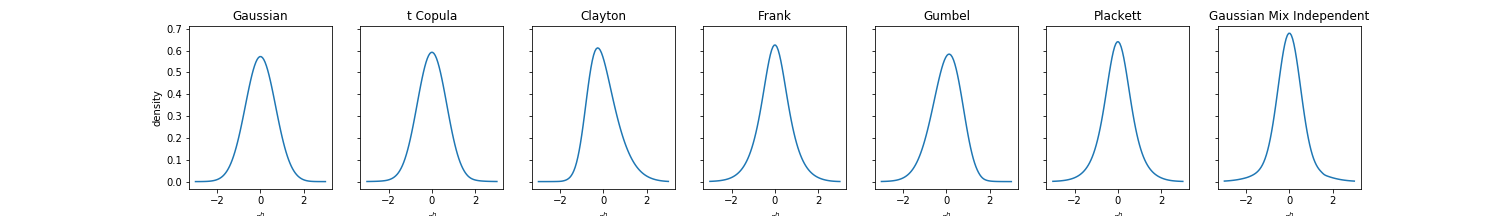
\includegraphics[width=\textwidth]{_pics/density illustration1.png}
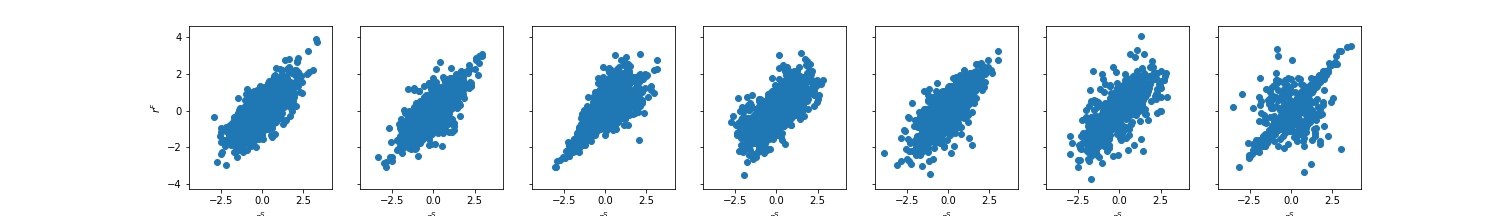
\includegraphics[width=\textwidth]{_pics/density illustration2.png}
  \caption{Upper Panel: Density of $Z= X - hY$ of different copulas with
  $X, Y \sim N(0,1)$,
  $0.75$ Spearman's rho between $X$ and $Y$, and $h=0.5$;
  Lower Panel: Scatter plot of samples from copulas.
  This illustration shows how dependence structure modelled by different copulas affects the density of the linear combination
  of margins.
  Notice that the $Z$ modelled by the asymmetric copulas, namely the Clayton and Gumbel copulas, are skewed to right
  and left respectively.}
\label{fig:density illustration}
\end{figure}
  % \begin{align*}
  %   C(u,v) &=\int_0^1 \frac{\partial}{\partial u} C(u,v)\, \dd u %
  %            = \int_0^1 \frac{\partial}{\partial u} \p(U\leq u, V\leq v)\, \dd
  %            u \\ %
  %          &= \int_0^1 \p(U\in \dd u, V\leq v)\, \dd u %
  %            = \int_0^1 \p(V\leq v|U=u) \underbrace{\p(U\in \dd
  %            u)}_{=1}\, \dd u\\
  %          &= \int_0^1 \p(V\leq v|U=u) \, \dd u %
  %            % = \int_\R \p(F_Y(Y)\leq F_Y(y) |F_X(X) = F_X(x))\, \dd
  %            % F_X(x) \\
  %          = \int_\R \p(F_Y(Y)\leq F_Y(y) |F_X(X) = F_X(x))\, f_X(x) \dd
  %            x %
  %            = \int_\R \p(Y\leq y|X=x)\, f_X(x) \dd x.
  % \end{align*}
  % Consequently $\displaystyle \frac{\partial}{\partial u} C(u,v) =
  % \frac{\partial}{\partial F(x)} C(F(x), F(y)) = \p(Y\leq y|X=x)$
  % $\pas$.

\subsection{Spectral Risk Measures}\label{subsec:spectral-risk-measures}
Spectral Risk Measures takes a form of

\begin{equation}\label{eq:SRM}
	M_{w}(X)=- \int^1_{0} w(p)q_{s}(X)ds
	\end{equation}\\

\noindent where $w(p)$ is a weighting function defined over the full range of cumulative probabilities $p \in [0,1]$. $M_{w}$ is a coherent measure if and only if $w$ satisfies, \\

\begin{itemize}
			\item Nonnegativity: $w(p) \ge 0$.
			\item Increasingness: $w'(p) \ge 0$.
			\item Normalisation: $\int^1_{0}w(p)dp=1$.
\end{itemize}
The first property requires that the weights are non-negative, and the second property is intended to reflect user risk aversion. The third one requires that the probability-weighted weights should sum to 1. %However, a drawback with property 3 is that it does not rule out the ES from the set of SRMs. In this case, we use the following property with strong condition instead of the third one. \\
\begin{itemize}
			\item Strict increasingness: $w'(p) > 0$.
\end{itemize}

\noindent Note that VaR and ES are included to spectral risk measure as special cases. The weighting function of VaR is a Dirac delta function which gives the outcome an infinite weight and the others a zero weight. On the other hand, the ES gives all tail quantiles the same weight. Both of them are not a suitable weight function for capturing investor's risk attitudes. \\

By setting a 'well-behaved' risk-aversion function which indicates the weights will rise more rapidly when the degree of risk aversion is higher, we investigate the behaviors of the users in terms of different weight function when they determine the hedge ratios. \\

We also consider wildly used risk measure is Value at Risk, VaR, a quantile of the portfolio loss distribution ({\color{blue}\citealp{jurgen2011statistics}})
\begin{equation}\label{eq:VaR}
q_{\alpha}(X) = F^{-1}_{X}(\alpha), \quad \alpha \in (0,1).
\end{equation}\\
For any random variable $X$, and its cumulative distribution function $F_X$ is well defined.
Due to the inconsistency of coherent risk, the use of expected shortfall has been discussed intensively in finance and risk management ({\color{blue}\citealp{jurgen2011statistics}}). Expected shortfall (ES) measures are expressed as
\begin{equation}\label{eq:ES}
\mbox{ES}_{\alpha}(X) = \frac{1}{1-\alpha}\int^1_{\alpha}q_{s}(X)ds
\end{equation}\\

\subsection{Two Risk Spectra}
Recognising the importance of the weighting function, we investigate different utility functions, $U(x)$ defined over outcomes $x$. Consider the exponential utility and power utility, where the investor's coefficient of absolute risk aversion is $k(x)= -\frac{U''(x)}{U'(x)} $ and his relative risk-aversion is $\gamma(x)=-\frac{xU''(x)}{U'(x)}$. This allows us to transfer the utility function to a weighting function as in {\color{blue}\citet{dowd2008spectral}}.

\subsubsection{Exponential Spectral Risk Measure}
  The exponential SRM is specified by only one risk parameter $k$. To obtain the risk spectrum, we set $ w(p)= \lambda e^{-k(1-p)}$ and $\lambda = \frac{k}{1-e^{-k}}$. Then, the risk spectrum and its antiderivative are: 

\begin{equation}\label{eq:w}
 w(p)=\frac{ke^{-k(1-p)}}{1-e^{-k}},\quad \mbox{and} \quad  W(p)=-\frac{1-e^{-k(1-p)}}{1-e^{-k}}
\end{equation}\\

\noindent where $k \in (0, \infty),\quad p\in [0, 1]$. This function depends on only one $k$. Figure \ref{Fig1:EPSRM} shows the exponential risk spectrum and its antiderivative for $k=1$, and $2$. By substituting into (\ref{eq:SRM}), the exponential SRM is, 
\begin{equation}\label{eq:ESRM}
 M_{w}(X)= \int^1_{0} \frac{ke^{-k(1-p)}}{1-e^{-k}}F^{-1}(p)dp
\end{equation}

\subsubsection{Power Spectral Risk Measure}
The power weighting function only has one parameter, $\gamma$, which leads to $w(p)= \frac{\lambda (1-p)^{\gamma-1}}{1-\gamma}$ as $0<\gamma<1$. Then, by setting $\lambda =\gamma(1-\gamma)$, the risk spectrum and its antiderivative are, 
\begin{equation}\label{eq:wp}
 w(p)=\gamma(1-p)^{\gamma-1},\quad \mbox{and} \quad  W(p)=-(1-p)^{\gamma}
 \end{equation}\\
  Plugging the weighting function to (\ref{eq:SRM}), the power SRM is obtained,
 %By setting $\gamma= 0.5$ and $0.8$, power risk spectrum and its antiderivative are showed in Figure \ref{Fig2:PSRM}.  
 \begin{equation}\label{eq:PSRM}
 M_{w}(X)= \int^1_{0} \gamma(1-p)^{\gamma-1}F^{-1}(p)dp
\end{equation}
 For the case of $\gamma >1$, we have $w(p)= \frac{\lambda p^{\gamma-1}}{1-\gamma}$ with $\lambda =\gamma(1-\gamma)$. The risk spectrum is written as, 
\begin{equation}\label{eq:wp2}
 w(p)= \gamma p^{\gamma-1} 
\end{equation}\\
The Power SRM then becomes,
\begin{equation}\label{eq:PSRM2}
 M_{w}(X)= \int^1_{0} \gamma p^{\gamma-1}F^{-1}(p)dp
 \end{equation}\\

\begin{figure}
	\begin{center}
		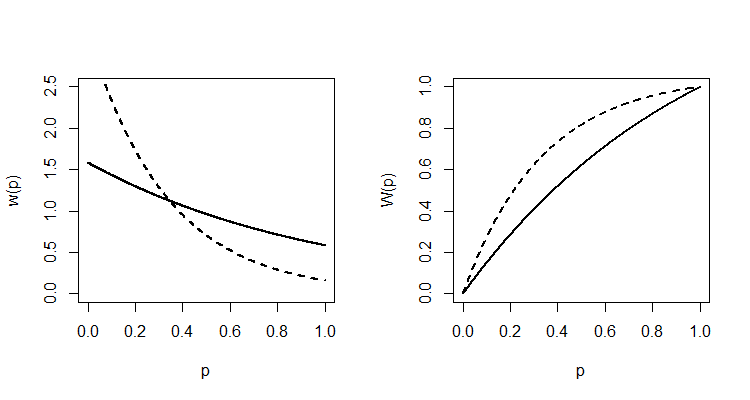
\includegraphics[scale = 0.7]{Figures/Fig1-1.png}\\
		%\vspace*{-10pt}\quantnet \href{https://github.com/mangrou/SRM/blob/master/SRM_QF/SRM_QF.m}{SRM\_QF} 
	\end{center}
	\caption{Exponential SRMs for $k=1$ (dashed) and $k=2$ (solid).}\label{Fig1:EPSRM}
\end{figure}

\begin{figure}
	\begin{center}
		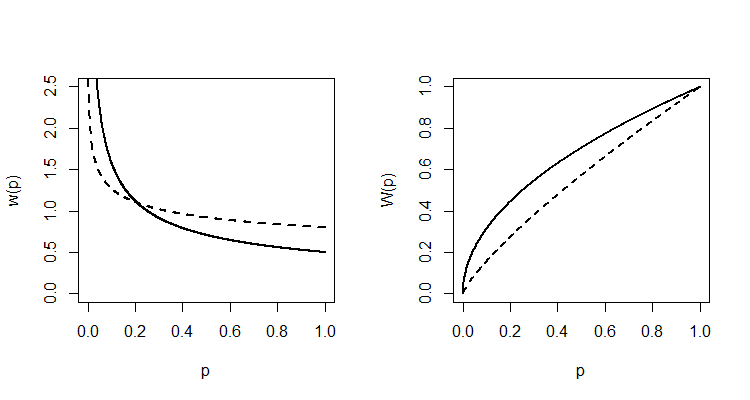
\includegraphics[scale = 0.7]{Figures/Fig2-1.png}\\
		%\vspace*{-10pt}\quantnet \href{https://github.com/mangrou/SRM/blob/master/SRM_QF/SRM_QF.m}{SRM\_QF} 
	\end{center}
	\caption{Power SRMs for $\gamma=0.5$ (solid) and $\gamma=0.8$ (dashed).}\label{Fig2:PSRM}
\end{figure}		
%%\subsubsection{Critical Parameter Region}
%%Following {\color{blue}\citet{brandtner2015decision}}, we try to restrict the relevant risk parameters $k$ and $\gamma$ which fall in the regions of strong risk aversion. The lower bound of risk parameter of exponential SRM, $k$, is set to $1.5937$ and $\gamma=$ is $0.5$ for power SRM.   {\color{blue}\citet{loomes1988different}} indicates the lower bound corresponds to a risk parameter of $k=5.7$ for exponential SRM measure, and of $\gamma= 0.115$ for power SRM for the binary lottery. {\color{blue}\citet{harrison2008risk}} indicate an average EU-function based on pooled utility function to yield $k=3.09$ and $\gamma= 0.37$. The parameters estimated from both literatures are lying in the problematic region of risk aversion. \\
%%
%%This paper discovers the hedge ratio is becoming less although he is ranked more risk averse that the risk aversion parameter of exponential SRM is beyond $1.5$. Moreover, if the risk aversion parameter of power SRM is beyond $0.8$, the hedge ratio becomes less. This empirical result is in line with the points of {\color{blue}\citet{brandtner2015decision}}.
%% 
%%Although those literatures provide the theoretical results of the threshold, this paper discovers the hedge ratio is becoming less although he is ranked more risk averse by minimizing exponential SRMs of the joint distribution of S\&P 500 spot and futures if risk aversion parameter beyond $9.8$. This result provides the reference of threshold to the risk aversion parameters in line with the points of {\color{blue}\citet{brandtner2015decision}}.
%
%
%
%
%\subsection{The Optimal Hedge Ratio}
%
%The optimal hedge ratio is defined as the ratio of the futures position to hedge the down size risk of selling one corresponding stock in the future ({\color{blue}\citealp{hull2016options}}). The hedge portfolio is: 
%
%\begin{equation*}
%        r_p=(r_s-\chi r_f)
%     \end{equation*}
%\noindent where $r_s$ and $r_f$ are denoted the return on the spot and the futures position, respectively. $\chi$ indicates the daily hedge ratio. Following {\color{blue}\citet{barbi2014copula}}, our purpose is to model the quantiles of $r_p$, where the dependence structure between $r_s$ and $r_f$ is modeled by a copula function, $C$. The $F^{-1}_{r_p}(\alpha)$ solves the following, 
%\begin{equation}\label{eq:QF}
%       1- \int^1_{0}  \frac{\partial }{\partial u} C\left[ u,1-F_{r_f} \left\lbrace \frac{F^{-1}_{r_p}(\alpha) - F^{-1}_{r_s}(u)}{\chi}\right\rbrace \right]  du=\alpha
%     \end{equation}
%
%\noindent The density of the copula is presented as, 
%\begin{equation}\label{eq:QFdensity}
% \int^1_{0} c\left[ u,1-F_{r_f} \left\lbrace \frac{F^{-1}_{r_p}(\alpha) - F^{-1}_{r_s}(u)}{\chi}\right\rbrace \right]  f_{r_p}\left\lbrace \frac{F^{-1}_{r_p}(\alpha) - F^{-1}_{r_s}(u)}{\chi}\right\rbrace du=f_{r_p}(\alpha)
%     \end{equation}
%\noindent where $f_{r_p}(x)=\frac{\partial }{\partial x}F_{r_p}(x)$. Equation (\ref{eq:QF}) defines the quantile function $F^{-1}_{r_p}(\alpha)$ implicitly. Thus, the optimal hedge ratio, $\chi$, is determined as, 
%
%\begin{equation}\label{eq:optimal}
%\hat{\chi}=\mbox{arg}\min_{\chi} M_{w}(r_p)	
%\end{equation}
%
%
%
%\section{Data}
%%\subsection{Financial Data}
%%
%%In this section, we illustrate how to proceed with the financial data. By assuming the S\&P 500 index and it corresponding futures index, S\&P 500 futures following the EGARCH(1,1),   
%%
%%\begin{equation*}
%%\begin{aligned}
%%&r_{i,t}=a_i+b_ir_{i,t-1}+\varepsilon_{i,t}.\\
%%&\varepsilon_{i,t} 
%%\mid \Omega_{t-1}= h_{i,t}z_{i,t}.\\
%%&z_{i,t}\sim iid\hspace{2mm}t_i.\\
%%&h^2_{i,t}=exp\{c_i+m_i\mbox{log}h^2_{i,t-1}+\beta_iz_{i,t-1}+\theta[\vert z_{i,t-1}\vert-\mathsf{E}(\vert z_{i,t-1}\vert)]\}.\\
%%&i=\{s,f\}.\\
%%\end{aligned}
%%\end{equation*}
%%
%%\noindent where $r_{i,t}$ are retuns and $\varepsilon_{i,t}$ are i.i.d vectors. By applying the different copulae, the parameters are computed from the EGARCH filtered data. 
%
%\subsection{Data Description}
%
%To demonstrate the application of copulae in optimal hedge ratio estimation, we collect daily data on six stock indices (FTSE 100, FTSE Mid 250, FTSE 350 and S\&P 500, S\&P Composite 1500 for the US market) and  two exchange rates (EURUSD and EURGBP). We use the FTSE 100 futures to hedge the spot position on all UK indices; the S\&P 500 to hedge the spot position on both US indices; currency futures on EURUSD and EURGBP to hedge the repective currency spot position. We draw daily data from Bloomberg and collect around 30 years of dat from January 1990 as possible. This is feasible for all UK spot and futures indices, for S\&P 500 spot and futures index. For the remaining series, we select the maximum spot and futures paired common time period, that is for currencies. Our dataset begins on 11 January 1999 (the euro was introduced as an accounting currency on 1 January 1999). For S\&P,  Composite 1500 it starts on 30 December 1994. 
%In total, we at most obtained 7898 pairs of daily observations for the index and index futures from 1999 to 2019 from Bloomberg. Futures prices are considered as a continuous series, by rolling over maturity on the first day of the delivery month. This is a common practice when dealing with futures data. ({\color{blue}\citealp{carchano2009rolling}}).
%Regardless of the maturities of futures price time series, the descriptive statistics are presented in Table \ref{TB1:Summary}. It reports the sample descriptive statistics. The summary statistics shows that they are skewed to the left except currency EURGBP, and the kurtosis coefficients are all greater than three except currency EURUSD which means heavy-tailed distribution. In particular, among stock indices, S\&P exhibits the highest kurtosis. The result is showing that the financial data is far from being Gaussian. \\
%Table \ref{TB2} shows the time-varying correlations between spot and futures series during the considered time period. On average, looking at the time period as a whole, correlations are generally high. UK and US stock indinces report an average correlation of about $97\%$, except for the FTSE 250 index, which correlates the less with the FTSE 100 futures ($78\%$). The average correlation diminishes as we pass to consider exchange rates ($94\%$ and $95\%$ for EURUSD and EURGBP, respectively).  However, the most important insight from Table \ref{TB2} is that correlations are not constant over time. Specifically, correlations are generally lower during the 199s and increase dramatically afterwards. 
%
%
%\begin{table}[ht]
%	\centering
%	\resizebox{\textwidth}{25mm}{
%	\begin{tabular}{lrrrrrrrr}
%		\hline
%		Spot & N & Average(\%) & SD(\%) & Minimum(\%) & Median(\%) & Maximum(\%) & Skewness & Kurtosis \\ 
%		\hline
%		S\&P 500 &  7898 & 0.0113 & 0.4890 & -5.5439 & 0.0113 & 4.7586 & -0.3968 & 12.2127 \\ 
%		S\&P 1500 &  6595 & 0.0121 & 0.5162 & -5.6081 & 0.0158 & 4.6787 & -0.4447 & 11.5959 \\ 
%		FTSE 100 &  7898 & 0.0047 & 0.4737 & -4.9998 & 0.0013 & 4.0756 & -0.2915 & 8.2525 \\ 
%		FTSE 250 &  7898 & 0.0099 & 0.4074 & -4.2649 & 0.0202 & 3.4912 & -0.5345 & 9.7249 \\ 
%		FTSE 350 &  7898 & 0.0054 & 0.4524 & -4.8701 & 0.0061 & 3.8882 & -0.3429 & 8.7289 \\ 
%		EURUSD &  7898 & -0.0006 & 0.2647 & -1.4687 & 0.0000 & 1.4986 & -0.0076 & 1.9539 \\ 
%		EURGBP &  7898 & 0.0008 & 0.2387 & -1.3604 & -0.0033 & 2.6109 & 0.2390 & 3.7460 \\ 
%		\hline
%		Futures &  &  & & & & & & \\ 
%		 \hline
%		S\&P 500 &  7898 & 0.0111 & 0.4972 & -4.7571 & 0.0157 & 5.7315 & -0.2701 & 12.6629 \\ 
%		FTSE 100 &  7898 & 0.0046 & 0.4929 & -4.3790 & 0.0000 & 4.1607 & -0.2581 & 6.7389 \\ 
%		FTSE 250 &  1647 & 0.0013 & 0.4288 & -4.0818 & 0.0149 & 3.2992 & -1.3365 & 18.3208 \\ 
%		EURUSD &  5712 & -0.0002 & 0.2589 & -1.3276 & 0.0000 & 1.4281 & -0.0282 & 1.6687 \\ 
%		EURGBP &  5543 & 0.0017 & 0.2174 & -1.5530 & 0.0000 & 2.6138 & 0.4844 & 7.2533 \\ 		
%		\hline\hline
%	\end{tabular}
%}
%\caption{{Descriptive Statistics for the sample of spot and futures returns}\\ Daily prices are taken from Bloomberg. Sample periods are from January 1990-December 2019 (UK indices, S\&P 500), while the start date is postponed to January 1995 for S\&P Composite 1500, January 1999 for currencies. }\label{TB1:Summary}
%\end{table}
%
%
%
% \begin{table}[h!]
%		\begin{center}
%			\resizebox{\textwidth}{25mm}{
%			\begin{tabular}{lrrrrrrrr}
%				\hline\hline
%				Spot & Futures & 1990-2019 & 1990-1994 & 1995-1999 & 2000-2004 & 2005-2009 & 2010-2014 & 2015-2019 \\
%				 \hline
%				S\&P 500 & S\&P 500 & 0.980& 0.964 & 0.961 & 0.972 & 0.982 & 0.980 & 0.980 \\ 
%				S\&P 1500 & S\&P  500 & 0.980 & - & 0.958 & 0.971 & 0.981 & 0.980 & 0.980 \\
%				FTSE 100 & FTSE 100 & 0.970 & 0.921 & 0.961 & 0.975 & 0.985 & 0.970 & 0.970 \\ 
%				%FTSE 100 & FTSE 250 & 0.780 & - & - & - & - & 0.780 & 0.780 \\ 
%				FTSE 250 & FTSE 100 & 0.780 & 0.751 & 0.647 & 0.694 & 0.854 & 0.880 & 0.780 \\ 
%				FTSE 250 & FTSE 250 & 0.980 & - & - & - & - & 0.970 & 0.980 \\ 
%				FTSE 350 & FTSE 100 & 0.960 & 0.917 & 0.957 & 0.974 & 0.984 & 0.970 & 0.960 \\ 
%				FTSE 350 & FTSE 250 & 0.830 & - & - & - & - & 0.830 & 0.830 \\ 
%				EURUSD & EURUSD & 0.940 & - & - & 0.947& 0.935 & 0.930 & 0.940 \\ 
%				EURGBP & EURGBP & 0.950 & - & - & 0.731 & 0.956 & 0.960 & 0.950\\   
%				\hline \hline
%			\end{tabular}
%		}
%		\end{center}
%		\caption{{Average correlations between spot and futures daily returns over time, and the overall average correlation over the considered time (1990-2014, except for the S\&P Composite 1500, currencies. )}\\
%                 SD stands for standard deviation}\label{TB2}
%	\end{table}	
%\begin{sidewaystable}[h]
%
%	\centering
%	\resizebox{\textwidth}{25mm}{
%	\begin{tabular}{llrrrrrrrrrrrrrrrr}
%		\hline\hline
%		&&k=10&&&&k=50&&&&k=100&&&&k=200\\
%		\hline
%		Spot & Futures & Gaussian & t & Clayton & Frank & Gaussian & t & Clayton & Frank & Gaussian & t & Clayton & Frank & Gaussian & t & Clayton & Frank \\ 
%		\hline
%	S\&P 500 & S\&P 500 & 0.912 & 0.912 & 0.930 & 0.912 & 0.912 & 0.850 & 0.912 & 0.904 & 0.912 & 0.912 & 0.912 & 0.912 & 0.896 & 0.896 & 0.896 & 0.945 \\ 
%	S\&P 1500 & S\&P  500 & 0.860 & 0.831 & 0.838 & 0.821 & 0.817 & 0.813 & 0.817 & 0.817 & 0.830 & 0.830 & 0.830 & 0.830 & 0.886 & 0.813 & 0.813 & 0.824 \\ 
%	FTSE 100 & FTSE 100 & 1.078 & 1.078 & 1.069 & 1.021 & 1.072 & 1.072 & 1.050 & 1.120 & 1.083 & 1.083 & 1.129 & 1.064 & 1.064 & 1.064 & 1.064 & 1.079 \\ 
%	FTSE 250 & FTSE 100 & 1.025 & 1.025 & 1.064 & 1.078 & 1.061 & 1.061 & 1.059 & 1.030 & 1.072 & 1.072 & 1.064 & 1.064 & 1.074 & 1.074 & 1.074 & 1.018 \\ 
%	FTSE 250 & FTSE 250 & 0.844 & 0.844 & 0.844 & 0.721 & 1.057 & 1.057 & 1.057 & 0.844 & 1.127 & 1.127 & 1.127 & 0.897 & 0.844 & 0.844 & 0.844 & 0.844 \\ 
%	FTSE 350 & FTSE 100 & 1.064 & 1.064 & 1.074 & 1.064 & 1.021 & 1.021 & 1.038 & 1.022 & 1.014 & 1.014 & 1.030 & 1.029 & 1.067 & 1.067 & 1.073 & 1.071 \\ 
%	FTSE 350 & FTSE 250 & 1.127 & 1.127 & 0.844 & 0.844 & 0.844 & 0.844 & 0.844 & 0.844 & 0.844 & 0.844 & 0.844 & 0.844 & 0.844 & 0.844 & 1.054 & 0.844 \\ 
%	EURUSD & EURUSD & 0.884 & 0.884 & 1.016 & 1.049 & 0.990 & 0.990 & 1.049 & 1.012 & 1.007 & 1.007 & 1.024 & 1.094 & 1.073 & 1.073 & 1.119 & 1.073 \\ 
%	EURGBP & EURGBP & 0.875 & 0.875 & 0.946 & 0.821 & 0.868 & 0.868 & 0.839 & 0.839 & 0.868 & 0.868 & 0.899 & 0.899 & 0.851 & 0.851 & 0.878 & 0.878 \\ 
%	\hline\hline
%	\end{tabular}
%
%}
%\caption{{ Risk measures ERM whose risk spectrum is computed as $\frac{ke^{-k(1-p)}}{1-e^{-k}}$ for different values of the risk-aversion parameter, $k=10,50,100, 200$. Optimal hedge ratios are numerically computed by employing Gaussian, t, Clayton, and Frank coupla within the interval $\chi \in [0,2]$. }}\label{TB3}
%\end{sidewaystable}
%
%\begin{sidewaystable}[h]
%
%	\centering
%		\resizebox{\textwidth}{25mm}{
%	\begin{tabular}{llrrrrrrrrrrrrrrrr}
%		\hline\hline
%		&&k=10&&&&k=50&&&&k=100&&&&k=200\\
%		\hline
%		Spot & Futures & Gaussian & t & Clayton & Frank & Gaussian & t & Clayton & Frank & Gaussian & t & Clayton & Frank & Gaussian & t & Clayton & Frank \\ 
%		\hline
%S\&P 500 & S\&P 500 & 33.814 & 38.798 & 28.364 & 31.132 & 54.568 & 59.986 & 55.437 & 60.220 & 74.920 & 70.001 & 89.273 & 76.559 & 80.241 & 91.317 & 71.773 & 88.429 \\ 
%S\&P 1500 & S\&P  500 & 22.871 & 32.999 & 28.563 & 17.658 & 69.911 & 61.774 & 51.861 & 77.193 & 85.481 & 78.789 & 87.087 & 86.246 & 93.169 & 91.844 & 86.655 & 89.643 \\ 
%FTSE 100 & FTSE 100 & 33.584 & 25.058 & 16.770 & 28.116 & 61.403 & 64.668 & 74.499 & 55.733 & 71.349 & 50.023 & 66.138 & 79.556 & 68.978 & 95.682 & 84.758 & 74.778 \\ 
%FTSE 250 & FTSE 100 & 30.084 & 34.479 & 19.898 & 31.599 & 61.803 & 51.637 & 83.963 & 58.590 & 67.908 & 81.406 & 68.085 & 71.678 & 87.258 & 95.253 & 94.100 & 83.709 \\ 
%FTSE 250 & FTSE 250 & 30.321 & 30.895 & 33.360 & 14.903 & 74.442 & 66.565 & 68.999 & 68.434 & 68.089 & 84.845 & 63.363 & 78.544 & 46.787 & 71.227 & 82.487 & 68.748 \\ 
%FTSE 350 & FTSE 100 & 21.101 & 38.074 & 17.215 & 30.615 & 66.373 & 76.581 & 50.438 & 80.746 & 85.867 & 87.246 & 84.649 & 70.232 & 84.797 & 94.362 & 81.758 & 89.652 \\ 
%FTSE 350 & FTSE 250 & 17.537 & 18.910 & 24.017 & 28.306 & 71.080 & 70.428 & 55.334 & 64.546 & 70.772 & 82.099 & 75.778 & 83.707 & 79.084 & 75.809 & 93.772 & 86.089 \\ 
%EURUSD & EURUSD & 31.562 & 33.946 & 33.480 & 36.584 & 65.384 & 73.455 & 69.224 & 71.995 & 81.246 & 72.280 & 73.939 & 84.373 & 86.337 & 88.065 & 90.596 & 89.791 \\ 
%EURGBP & EURGBP & 26.448 & 22.900 & 15.944 & 12.199 & 63.195 & 63.663 & 57.152 & 70.825 & 83.902 & 80.827 & 83.990 & 82.230 & 82.992 & 87.950 & 83.966 & 84.220 \\ 
%\hline\hline
%	\end{tabular}
%}
%\caption{{ Risk measures ERM whose risk spectrum is computed as $\frac{ke^{-k(1-p)}}{1-e^{-k}}$ for different values of the risk-aversion parameter, $k=10,50,100, 200$. Hedging effectiveness is measured as the percentage reduction of portfolio risk attributable to hedging, that is 1 minus the ratio between the risk of the optimally hedged portfolio and the risk of the unhedged portfolio.}}\label{TB4}
%
%\end{sidewaystable}
%
%
%
%\begin{sidewaystable}[h]
%	
%	\centering
%	\resizebox{\textwidth}{25mm}{
%		\begin{tabular}{llrrrrrrrrrrrrrrrr}
%			\hline\hline
%			&&k=10&&&&k=50&&&&k=100&&&&k=200\\
%			\hline
%			Spot & Futures & Gaussian & t & Clayton & Frank & Gaussian & t & Clayton & Frank & Gaussian & t & Clayton & Frank & Gaussian & t & Clayton & Frank \\ 
%			\hline
%			S\&P 500 & S\&P 500 & 1.699 & 1.699 & 1.699 & 1.699 & 1.699 & 1.699 & 1.699 & 1.815 & 1.749 & 1.749 & 1.749 & 1.749 & 1.247 & 1.247 & 1.247 & 1.602 \\ 
%			S\&P 1500 & S\&P  500 & 1.506 & 1.506 & 1.506 & 1.488 & 1.502 & 1.502 & 1.502 & 1.502 & 1.564 & 1.564 & 1.564 & 1.656 & 1.456 & 1.456 & 1.456 & 1.293 \\ 
%			FTSE 100 & FTSE 100 & 1.533 & 1.533 & 1.533 & 1.533 & 1.533 & 1.533 & 1.533 & 1.533 & 1.162 & 1.162 & 1.162 & 1.533 & 1.575 & 1.544 & 1.575 & 1.533 \\ 
%			FTSE 250 & FTSE 100 & 1.533 & 1.533 & 1.533 & 1.533 & 1.533 & 1.533 & 1.533 & 1.533 & 1.533 & 1.533 & 1.178 & 1.533 & 0.718 & 1.544 & 1.575 & 1.533 \\ 
%			FTSE 350 & FTSE 100 & 1.533 & 1.463 & 1.533 & 1.533 & 1.355 & 1.463 & 1.533 & 1.533 & 0.842 & 0.842 & 0.842 & 1.533 & 1.575 & 1.544 & 1.575 & 1.533 \\ 
%			EURUSD & EURUSD & 1.792 & 1.792 & 1.842 & 1.792 & 1.792 & 1.792 & 1.792 & 1.792 & 1.660 & 1.124 & 1.660 & 1.660 & 1.792 & 1.792 & 1.792 & 1.792 \\ 
%			EURGBP & EURGBP & 1.803 & 1.803 & 1.803 & 1.803 & 1.803 & 1.803 & 1.803 & 1.803 & 1.803 & 1.803 & 1.803 & 1.803 & 1.803 & 1.803 & 1.803 & 1.803 \\ 
%			\hline\hline
%		\end{tabular}
%		
%	}
%	\caption{{ Risk measures ERM whose risk spectrum is computed as $\frac{ke^{-k(1-p)}}{1-e^{-k}}$ for different values of the risk-aversion parameter, $k=10,50,100, 200$. Optimal hedge ratios are numerically computed by employing Gaussian, t, Clayton, and Frank coupla within the interval $\chi \in [0,2]$ during 2007-2008. }}\label{TB5}
%\end{sidewaystable}
%
%\begin{sidewaystable}[h]
%	
%	\centering
%	\resizebox{\textwidth}{25mm}{
%		\begin{tabular}{llrrrrrrrrrrrrrrrr}
%			\hline\hline
%			&&k=10&&&&k=50&&&&k=100&&&&k=200\\
%			\hline
%			Spot & Futures & Gaussian & t & Clayton & Frank & Gaussian & t & Clayton & Frank & Gaussian & t & Clayton & Frank & Gaussian & t & Clayton & Frank \\ 
%			\hline
%			S\&P 500 & S\&P 500 & 36.993 & 27.857 & 18.408 & 20.172 & 69.464 & 31.418 & 44.283 & 68.940 & 89.510 & 77.586 & 69.902 & 80.468 & 80.919 & 95.673 & 82.801 & 93.582 \\ 
%			S\&P 1500 & S\&P  500 & 28.313 & 10.025 & 10.692 & 22.406 & 66.619 & 68.904 & 65.922 & 63.782 & 86.180 & 81.198 & 90.368 & 77.818 & 91.574 & 77.003 & 74.282 & 75.102 \\ 
%			FTSE 100 & FTSE 100 & 29.104 & 23.124 & 21.901 & 33.026 & 87.537 & 67.005 & 57.399 & 74.268 & 63.581 & 79.343 & 90.640 & 78.584 & 90.075 & 79.884 & 93.625 & 88.849 \\ 
%			FTSE 250 & FTSE 100 & 29.126 & 25.574 & 30.508 & 16.006 & 55.524 & 70.432 & 61.857 & 68.255 & 74.676 & 90.072 & 77.292 & 66.480 & 84.160 & 86.309 & 76.883 & 83.903 \\ 
%			FTSE 350 & FTSE 100 & 38.841 & 29.541 & 19.498 & 30.711 & 77.274 & 69.313 & 79.618 & 77.289 & 61.829 & 74.697 & 64.267 & 83.610 & 86.917 & 87.438 & 85.821 & 86.363 \\ 
%			EURUSD & EURUSD & 15.752 & 32.076 & 25.045 & 17.088 & 60.903 & 67.348 & 50.829 & 61.143 & 82.536 & 83.228 & 44.783 & 67.427 & 79.179 & 75.343 & 91.407 & 93.630 \\ 
%			EURGBP & EURGBP & 14.636 & 21.775 & 13.228 & 19.811 & 79.253 & 75.383 & 73.598 & 77.228 & 75.944 & 71.064 & 80.766 & 67.496 & 82.077 & 91.392 & 79.982 & 90.076 \\ 
%			\hline\hline
%		
%		\end{tabular}
%	}
%	\caption{{ Risk measures ERM whose risk spectrum is computed as $\frac{ke^{-k(1-p)}}{1-e^{-k}}$ for different values of the risk-aversion parameter, $k=10,50,100, 200$. Hedging effectiveness is measured as the percentage reduction of portfolio risk attributable to hedging, that is 1 minus the ratio between the risk of the optimally hedged portfolio and the risk of the unhedged portfolio during 2007-2008.}}\label{TB6}
%	
%\end{sidewaystable}
%
%
%\section{Empirical Result}
%
%The hedged portfolio composed by a long spot position and an opposite futures position. We choose 4 different kinds of copulae, Gaussian, $t$, Clayton and Frank to capture the dependence structure between the spot and its corresponding futures. 
%%Within the Archimedean family, Clayton copula exhibits mass lower tail and less on the upper. Gumbel copula shows strong linkage on the upper, but also shows more variability and more mass in the lower tail.\\ 
%SRM composed of quantile function and weighting function as presented in eq.(\ref{eq:SRM}). By applying different copulas, it shows the quantile function derived from eq.(\ref{eq:QF}).  By setting different hedge ratios $\chi = 0.4, 0.5, 0.6$, Fig. \ref{Fig3:QF1} shows the quantile function by plugging 4 different copulae functions. By employing the value of $k$ from $1$ to $20$, the exponential SRM can be estimated. As can be seen in Figure 4, the more risk averse $k$ becomes, the higher spectral risk it measures. However, the solid lines ($\chi = 0.4$) by conducting 4 different copulae will shift inward which indicates that spectral risk measurement goes lower when hedge ratio is high.\\
%%On the other hand, power SRM is also estimated by restricting $0<\gamma < 1$. Looking at the relationship between $\gamma$ and power SRM in Fig. \ref{Fig5:PSRM_r}, the power SRM declines while $\gamma$ is increasing in $(0,1)$. Although the dashed line ($\chi = 0.4$) is below the solid line ($\chi = 0.3$), in this case, the risk measurement subsequently falls as the user becomes more risk aversion that is odd. On the other hand, if $\gamma >1$, the power SRM with respect to $\gamma$ is increasing in Fig \ref{Fig6:PSRM2_r}. \\
%
%Having a close look at the relationship between SRMs and hedge ratio in Fig. \ref{Fig5:ESRM_HR}, we set $k=5$ (solid) and $10$ (dashed), and estimate the exponential SRM by employing $\chi$ from $0$ to $1$. Fig. \ref{Fig5:ESRM_HR} shows that the minimum exponential SRM of portfolio is reached by selecting the optimal hedge ratio. It is reasonable that the dashed line represents more risk aversion ($k=10$) is lying above the solid line ($k=5$), the less risk aversion, as hedge ration is larger than $0.2$. This is a proper property to describe the investor behaviour.   \\
%
%The optimal hedge ratios are obtained by (\ref{eq:optimal}) based on the estimated joint probability distribution of index and futures conducted by different copulae. Table \ref{TB3}  shows that the optimal hedge ratios are derived by minimizing the exponential SRM in terms of different degrees of risk aversion coefficient, $k= 10, 50, 100, 200$ by employing different copulae. For each portfolio we compute the optimal hedge ratios using rolloing windows of length 260 trading days. The copula dependence parameter is re-estimated every 260 observation. 
%This procedure leads to 30 windows for S\&P500, and FTSE 100, FTSE250, and FTSE 100 ( this three UK indices with FTSE 100 futures), 20 windows for 2 exchange rates, and S\&P1500, and 6 windows for FTSE 250 and FTSE 350 with FTSE 250 futures. Table \ref{TB3} shows the average optimal hedge ratios of each portfolio.\\
%
%The hedging effectiveness of copula-based model applied to ESRM is presented inTable \ref{TB4}. We use $k= 10, 50, 100, 200$ as the ESRM absolute risk aversion parameter. There is a positive relationship between the absolute risk aversion and the hedging effectiveness. This is not surprising. Intuitively, as k increases, the more emphasis is attributed to negative events, and it is expected that hedgeing effectiveness is increased. \\
%
%Having a look at crisis period, the optimal hedge ratios are estimated during 2007-2008. The results are in Table \ref{TB5}. Compared with Table \ref{TB3}, the optimal hedge ratios in crisis period is generally higher than the ones in overall periods. 
%
%
%\begin{figure}
%\begin{center}
%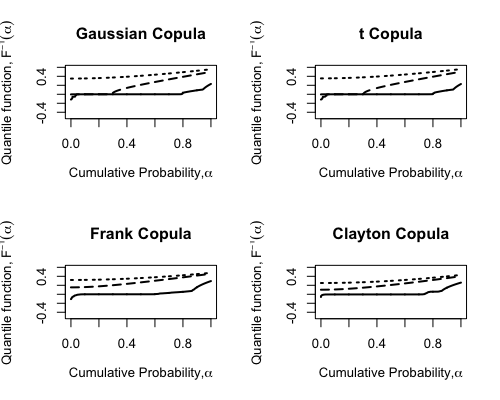
\includegraphics[scale = 0.75]{Figures/Fig3_20200726.png}\\
%%\vspace*{-10pt}\quantnet \href{https://github.com/mangrou/SRM/blob/master/SRM_QF/SRM_QF.m}{SRM\_QF} 
%\end{center}
%\caption{Setting $\chi = 0.4$ (solid), $0.5$ (dashed), and $0.6$ (dotted), quantile functions are estimated from (\ref{eq:QF}) by plugging Gaussian, $t$, Frank and Clayton copulae, respectively.}\label{Fig3:QF1}
%\end{figure}	
%
%
%%\begin{figure}
%%\begin{center}
%%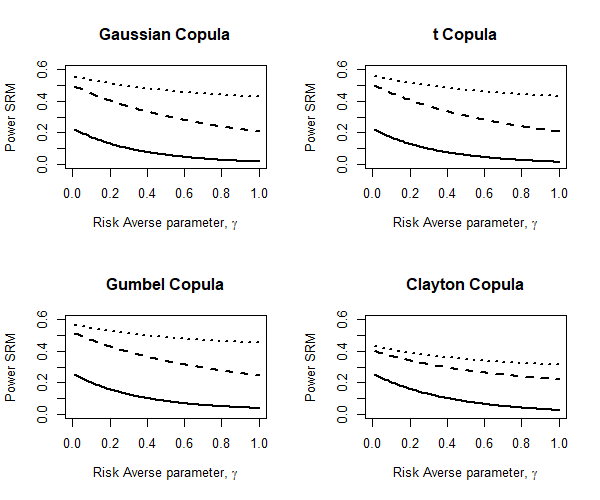
\includegraphics[scale = 0.8]{Figures/Fig5_20181001.png}\\
%%%\vspace*{-10pt}
%%%\quantnet \href{https://github.com/mangrou/SRM/tree/master/SRM}{ESRM} 
%%\end{center}
%%\caption{By setting setting $\chi = 0.4$ (solid), $0.5$ (dashed), and $0.6$ (dotted), power SRM is estimated from eq. (\ref{eq:PSRM}) as $0<\gamma<1$ by conducting Gaussian, $t$, Gumbel, Clayton copulae.}\label{Fig5:PSRM_r}
%%\end{figure}
%
%\begin{figure}
%\begin{center}
%	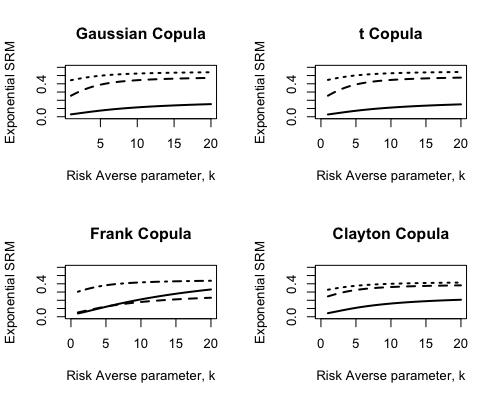
\includegraphics[scale = 0.75]{Figures/Fig5_20200726.png}\\
%	%\vspace*{-10pt}
%	%\quantnet \href{https://github.com/mangrou/SRM/tree/master/SRM}{ESRM} 
%\end{center}
% \caption{By setting $\chi = 0.4$ (solid), $0.5$ (dashed), and $0.6$ (dotted), exponential SRM is estimated from eq. (\ref{eq:ESRM}) by conducting Gaussian, $t$, Frank and Clayton copulae.}\label{Fig4}
%\end{figure}
%
%\begin{figure}
%\begin{center}
%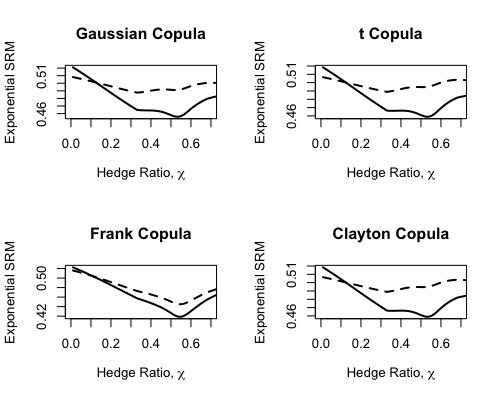
\includegraphics[scale = 0.8]{Figures/Fig6_20200726.png}\\
%%\vspace*{-10pt}
%%\quantnet \href{https://github.com/mangrou/SRM/tree/master/SRM}{ESRM} 
%\end{center}
%\caption{By setting $k = 5$ (solid) and $10$ (dashed), exponential SRM are estimated from (\ref{eq:ESRM}) by conducting Gaussian, $t$, Frank, Clayton copulae.}\label{Fig5:ESRM_HR}
%\end{figure}
%
% 
%   
%%\begin{figure}
%%\begin{center}
%%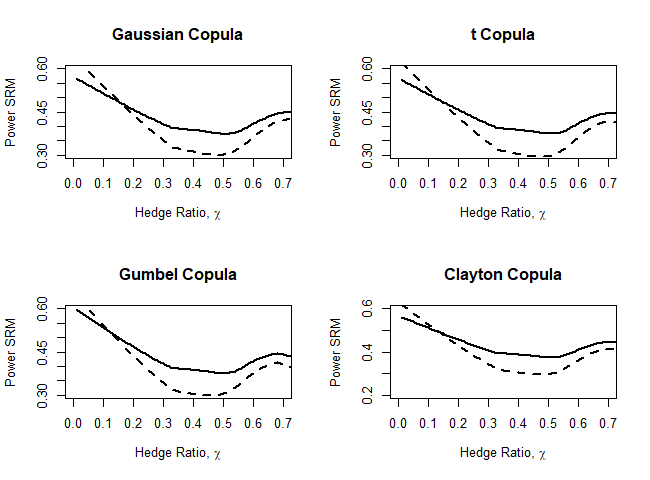
\includegraphics[scale = 0.8]{Figures/Fig8_20181002.png}\\
%%%\vspace*{-10pt}
%%%\quantnet \href{https://github.com/mangrou/SRM/tree/master/SRM}{ESRM} 
%%\end{center}
%%\caption{By setting $\gamma = 0.5$ (solid), $0.8$ (dashed), Power SRM is estimated from (\ref{eq:PSRM}) as $0<\gamma<1$ by conducting Gaussian, $t$, Gumbel, Clayton copulae}\label{Fig8:PSRM_HR}
%%\end{figure}
%
%
%%\begin{figure}
%%	\begin{center}
%%		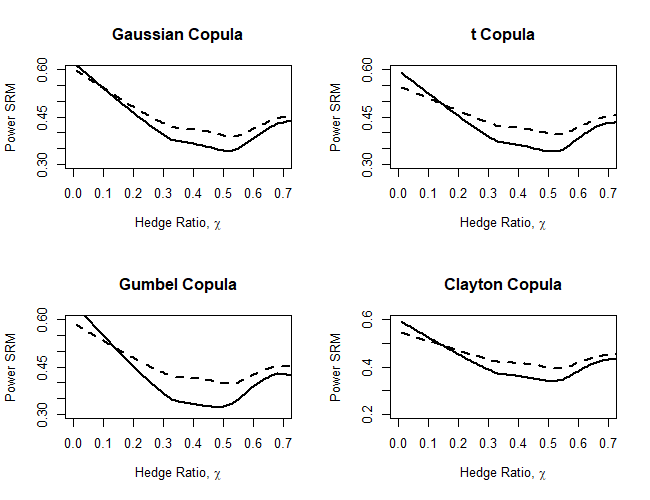
\includegraphics[scale = 0.8]{Figures/Fig9_20181002.png}\\
%%		%\vspace*{-10pt}
%%		%\quantnet \href{https://github.com/mangrou/SRM/tree/master/SRM}{ESRM} 
%%	\end{center}
%%	\caption{By setting $\gamma = 1.5$ (solid), $2$ (dashed), Power SRM is estimated from eq. (\ref{eq:PSRM2}) as $\gamma >1$ by conducting Gaussian, $t$, Gumbel, Clayton copulae}\label{Fig9:PSRM_HR}
%%\end{figure}
%
%
%
%
%
%
%
%\section{Conclusion}
%
%%We employ {\color{blue}\citet{barbi2014copula}} to illustrate the quantiles of the hedged portfolio in terms of a copula function. This method allows to estimate the hedged portfolio cumulative distribution function and separately choose the risk-minimizing hedge ratio. \\
%%
%%The general lesson of SRM is that users must be careful to ensure that utility functions should fit the features of the particular problems. By empirically investigating the relationship between the risk-aversion and the optimal hedge ratio, the exponential and power weighting function given $\gamma >1$ are more reasonable to illustrate the investors' risk attitude. The higher risk-averse it becomes the larger spectral risk it measures. 
%%%On the other hand, in our model, the optimal hedge ratio is much less successful to describe the investors behaviors. 
%%The higher risk measurement implies more willingness to pay for hedge ratio. As a consequence, these SRMs exhibit counter-intuitive results with respect to risk aversion. Spectral risk measurement is composed of the utility function of investor and the quantile function of assets. These two function will affect the investors behaviour. %To sum up, There is no conclusive summary about the optimal hedge ratio with respect to risk aversion parameter. \\ 
%%
%%This paper presents an approach to hedging with futures contracts which takes into two considerations that attract seldom adequate attention: Firstly, the quantiles of the hedged portfolio in terms of a copula function. Secondly, this paper implements different SRM by using empirical data to investigate which is reasonable to present the investors risk attitudes. Nonetheless, the results provide some sense of properties of different SRM applying to determine the optimal hedge ratio. \\
%
%%%%%%%%%%%%%%%%%%%%%%%%%%%%%%%%%%%%%%%%%%%%%%%%%%%%%%%%%%%%%%%%%%%%%%%%%
%


\documentclass[square]{article} %
\usepackage{amsfonts,amssymb,amsthm} %
\usepackage[tbtags]{amsmath} %
\usepackage{bm}
\newtheorem{theorem}{Theorem}
\newtheorem{prop}{Proposition}
\newtheorem{eg}{Example}


\begin{document}
    Copula is a function represent the multivariate structure of random variables.
    Frechet-Hoeffding lower bound $\bm{W}(u,v) = \min(u,v)$, Frechet-Hoeffding upper bound $\bm{M}(u,v) = \max(u+v-1,0)$,
    and product copula $\bm{\Pi}=uv$ are three important special instants of copulas.
    They describe the perfect counter-dependence, perfect dependence, and independence of two random variables, respectively.
    The inequality $\bm{W}(u,v) \leq \bm{C}(u,v) \leq \bm{M}(u,v)$ holds for every copula $\bm{C}$ ad every $(u,v) \in \mathbb{I}^2$ (Nelsen 2.2.5).

    \section{Ellpitical Copulas}\label{sec:ellpitical-copulas}
%    A random vector $X \in \mathbb{R}^d$ is said to have an elliptical distribution if it admits the stochastic representation
%    \begin{align}
%        \bm{X} = \bm{\mu}+ R\bm{A}\bm{U}
%        \end{align}
%where $\bm{\mu} \in \mathbb{R}^d$, $R$ is a positive random variable independent of $\bm{U}$,
%    $\bm{U}$ is a random vector uniform on the unit sphere in $\mathbb{R}^d$,
%    and $\bm{A}$ is a fixed $d \times d$ matrix such that $\bm{\Sigma} = \bm{A} \bm{A}^\intercal$ is non-singular.
%
%    The density function of an elliptical distribution is given by
%    \begin{align}
%        f(\bm{x}) = |\bm{\Sigma}|^{-\frac{1}{2}} g\{(\bm{x}-\bm{\mu})^\intercal \bm{\Sigma}^{-1}(\bm{x}-\bm{\mu})\}
%        \end{align}
%    for some function $g:\mathbb{R} \rightarrow \mathbb{R}^+$, the density generator.
%    The function g uniquely determine the distriution of $R$ (ref).
%
%    For multivariate Normal distribution, its density generator is
%    \begin{align}
%        g(t)=Ce^{-\frac{t}{2}}
%        \end{align}
%    where $C$ is .
%
%    For multivariate Student-t distribution, its density generator is
%        \begin{align}
%            g(t)=C\left(1+\frac{t}{m}\right)^{-\frac{d+m}{2}}
%        \end{align}
%
%%    An elliptical copula is .
%%    It can also be obtained by method of inversion (see)
%    If $H$ is a $d$-variate elliptical distribution, the corresponding elliptical copula is
%    \begin{align}
%        \bm{C}(\bm{u}) = H(F_{X_1}^{-1}(u_1),\dots, F_{X_d}^{-1}(u_d)).
%        \end{align}

    Elliptical copulas are copulas f elliptical distributions.
    Gaussian copula is the copula associated with multivariate normal distribution.
    The Gaussian copula (B1 in Joe) has a form
        \begin{align}
            \bm{C}(u,v) &= \Phi_{2, \rho}\{\Phi^{-1}(u), \Phi^{-1}(v)\} \\
                        &= \int_{-\infty}^{\Phi^{-1}(u)}
                           \int_{-\infty}^{\Phi^{-1}(v)}
                           \frac{1}{2\pi\sqrt{1-\rho^2}}
                           \exp{\left(
                           \frac{s^2-2\rho st+t^2}{2(1-\rho^2)}
                           \right)} ds dt
            \end{align}
    where $\Phi_{2, \rho}$ is the cdf of bivariate Normal distribution with zero mean, unit variance, and correlation $\rho$,
    and $\Phi^{-1}$ is quantile function univariate standard normal distribution.
    The copula density of Gaussian copula can be written as
    \begin{align}
        \bm{c}_\rho(u,v) &= \frac{\phi_{2,\rho}\{\Phi^{-1}(u), \Phi^{-1}(v)\}}
                            {\phi\{\Phi^{-1}(u)\} \cdot \phi\{\Phi^{-1}(v)\}}\\
                    &= \frac{1}{2\pi\sqrt{1-\rho^2}}\exp\left(
                       -\frac{u^2 - 2\rho uv + v^2}{2(1-\rho^2)}
                       \right) ,
        \end{align}
    where $\phi_{2,\rho}(\cdot)$ is the density of bivariate Normal distribution with zero mean,
    unit variance,
    and correlation $\rho$,
    and, $\phi(\cdot)$ the density of standard normal distribution.

    The Kendall's $\tau_K$ and Spearman's $\rho_S$ of a bivariate Gaussian Copula are
        \begin{align}
            \tau_K(\rho) = \frac{2}{\pi}\arcsin\rho
            \end{align}
        \begin{align}
            \rho_S(\rho) = \frac{6}{\pi}\arcsin\frac{\rho}{2}
            \end{align}

    t copula is associated with multivariate t distribution.
    The t Copula takes a form
    \begin{align}
            \bm{C}(u,v) &= \bm{T}_{2, \rho, \nu}\{T^{-1}_\nu(u), T^{-1}_\nu(v)\} \\
                &= \int_{-\infty}^{T^{-1}_\nu(u)}
                   \int_{-\infty}^{T^{-1}_\nu(v)}
                \frac{\Gamma\left(\frac{\nu+2}{2}\right)}
                {\Gamma\left(\frac{\nu}{2}\right)\pi\nu\sqrt{1-\rho^2}}\\
               & \left(
            1+\frac{s^2-2st\rho+t^2}{\nu}
            \right)^{-\frac{\nu+2}{2}} ds dt,
        \end{align}
    where $\bm{T}_{2, \rho, \nu}(\cdot, \cdot)$ denotes the cdf of bivariate t distribution with scale parameter $\rho$ and degree of free $\nu$,
    $T^{-1}_\nu(\cdot)$ is the quantile function of a standard t distribution with degree of freedom $\rho$.

    The copula density is
    \begin{align}
        \bm{c}(u,v) &= \frac{\bm{t}_{2, \rho, \nu}\{T^{-1}_\nu(u), T^{-1}_\nu(v)\}}
        {t_\nu\{T^{-1}_\nu(u)\}\cdot t_\nu\{T^{-1}_\nu(v)\}},
        \end{align}
    where $\bm{t}_{2,\rho, \nu}$ is the density of bivariate t distribution,
    and $t_\nu$ the density of standard t distribution.

    Like all the other elliptical copula, t copula's Kendall's $\tau$ is same to that of Gaussian copula (Demarta and reference therein).

    \section{Archimedean Copula}\label{sec:archimedean-copula}
    Archimedean copula forms a large class of copulas with many convenient features.

    In general, Archimedean copula takes a form
    \begin{align}
        \bm{C}(u,v)= \psi^{-1}\{\psi(u), \psi(v)\},
        \end{align}
    where $\psi:[0,1] \rightarrow [0,\infty)$ is a continuous, strictly decreasing and convex function such that
    $\psi(1)=0$ for any permissible dependence parameter $\theta$. $\psi$ is also called generator.
    $\psi^{-1}$ is the inverse the generator.

    This section will briefly introduce this class of copula,
    we refer readers to Nelsen and Joe for Detail of this class of copula.

    Frank copula (B3 in Joe) is a radial symmetric copula and does not have any tail dependence.
    It takes the form
    \begin{align}
        \bm{C}_{\theta}(u,v) &= \frac{1}{\log(\theta)}
        \log \left\{
        1 + \frac{(\theta^u-1)(\theta^v-1)}{\theta-1}
        \right\}
        \end{align}
    where $\theta \in [0, \infty]$ is the dependency parameter.
    $\bm{C}_1 = \bm{M}$, $\bm{C}_1 = \bm{\Pi}$, and $\bm{C}_\infty = \bm{W}$.

    The Copula density
    \begin{align}
        \bm{c}_{\theta}(u,v) &= \frac{(\theta-1)\theta^{u+v}\log(\theta)}
        {\theta^{u+v}-\theta^u-\theta^v+\theta}
        \end{align}

    Frank copula has Kendall's $\tau$ and Spearman's $\rho$ as follow:
    \begin{align}
        \tau_K(\theta) = 1-4\frac{D_1\{-\log(\theta)\}}{\log(\theta)},
        \end{align}
and
    \begin{align}
        \rho_S(\theta) = 1-12\frac{D_2\{-\log(\theta)\} - D_1\{\log(\theta)\}}{\log(\theta)},
        \end{align}
    where $D_1$ and $D_2$ are the Debye function of order 1 and 2.
    Debye function is $D_n = \frac{n}{x^n}\int_0^x\frac{t^n}{e^t-1}dt$.

    Gumbel copula (B6 in Joe) has upper tail dependence with the dependence parameter
    $\lambda^U = 2-2^{\frac{1}{\theta}}$ and displays no lower tail dependence.
    \begin{align}
        \bm{C}_{\theta}(u,v) &= \exp{-\{
        (-\log(u))^\theta +(-\log(v))^\theta
        \}^{\frac{1}{\theta}}},
        \end{align}
    where $\theta \in [1,\infty)$ is the dependence parameter.
    While Gumbel copula cannot model perfect counter dependence (ref), $\bm{C}_{1} = \bm{\Pi}$ models the independence,
    and $\lim\limits_{\theta \to \infty} \bm{C}_\theta = \bm{W}$ models the perfect dependence.

    The copula density takes the form
    \begin{align}
            f
        \end{align}

      \begin{align}
        \tau_K(\theta) =\frac{\theta-1}{\theta}
        \end{align}

    Clayton copula, opposite to Gumbel copula,
    generates lower tail dependence in a form $\lambda^L = 2^{-\frac{1}{\theta}}$,
    but generates no upper tail dependence.
    Clayton copula takes a form
    \begin{align}
        \bm{C}_{\theta}(u,v) &= \left[
        \max\{u^{-\theta}+v^{-\theta}-1,0\}\right]^{-\frac{1}{\theta}},
        \end{align}
    where $\theta \in (-\infty, \infty)$ is the dependency parameter.
    $\lim\limits_{\theta \to -\infty} \bm{C}_\theta = \bm{M}$, $\bm{C}_0 = \bm{\Pi}$, and $\lim\limits_{\theta \to \infty} \bm{C}_\theta = \bm{W}$.

    Its Kendall's $\tau$ is
    \begin{align}
        \tau_K(\theta) =\frac{\theta}{\theta+2}.
        \end{align}

    Plackett copula has an expression
    \begin{align}
        \bm{C}_{\theta}(u,v) &= \frac{1+(\theta-1)(u+v)}{2(\theta-1)}
                             - \frac{\sqrt{\{
        1+(\theta-1)(u+v)\}^2 - 4uv\theta(\theta-1)}}{2(\theta-1)}
        \end{align}
    \begin{align}
        \rho_S(\theta) = \frac{\theta+1}{\theta-1} - \frac{2\theta \log \theta}{(\theta-1)^2}
        \end{align}

    We include Placket copula in our analysis as it possesses a special property,
    the cross-product ratio is equal to the dependence parameter
    \begin{align}
        &\phantom{=} \frac{\mathbb{P}(U \leq u, V \leq v) \cdot \mathbb{P}(U > u, V > v)}
        {\mathbb{P}(U \leq u, V > v) \cdot \mathbb{P}(U > u, V \leq v)}\\
        &= \frac{C_\theta(u,v)\{1-u-v+C_\theta(u,v)\}}{\{u-C_\theta(u,v)\}\{v-C_\theta(u,v)}\\
        &= \theta.
        \end{align}
    That is, the dependence parameter is equal to the ratio between number of concordence pairs and number of discordence pairs of a bivariate random variable.
    \section{Mixture Copula}\label{sec:mixture-copula}
    Mixture copula is a linear combination of copulas.
    It allows us to model the dependence structure in a more flexible manner.

    For a 2-dimensional random variable $\bm{X}=(X_1,X_2)^\intercal$,
    its distribution can be written as linear combination $K$ copulas
    \begin{align}
        \mathbb{P}(X_1 \leq x_1, X_2 \leq x_2) = \sum_{k=1}^K p^k \cdot \bm{C}^{(k)}\{F^{(k)}_{X_1}(x_1;\bm{\gamma}^{(k)}_1),
        F^{(k)}_{X_2}(x_2;\bm{\gamma}^{(k)}_2); \bm{\theta^{(k)}}\}
        \end{align}
    where $p^{(k)} \in [0,1]$ is the weight of each component,
    $\bm{\gamma}^{(k)}$ is the parameter of the marginal distribution in the $k^\text{th}$ component,
    and $\bm{\theta^{(k)}}$ is the dependence parameter of the $k^\text{th}$ component.
    We also restrict the weight so that $\sum_{k=1}^K p^{(k)}=1$.
    Analysis of mixture copula with higher dimension can be found in Vrac et. al. (2011).

    We deploy a simplified version of the above representation by assuming the maringals of $\bm{X}$ are not mixture.
    By Sklar's theorem we write
    \begin{align}
        \bm{C}(u,v)= \sum_{k=1}^K p^{(k)} \cdot \bm{C}^{(k)}\{F^{-1}_{X_1}(u),
        F^{-1}_{X_2}(v); \bm{\theta^{(k)}}\}.
        \end{align}

    The copula density is again a linear combination of copula density
    \begin{align}
        \bm{c}(u,v)= \sum_{k=1}^K p^{(k)} \cdot \bm{c}^{(k)}\{F^{-1}_{X_1}(u),
        F^{-1}_{X_2}(v); \bm{\theta^{(k)}}\}.
        \end{align}

    While Kendall's $\tau$ of mixture copula is not known in close form,
    the Spearman's $\rho$ is

    \begin{prop}
        Let $\rho_S^{(k)}$ be the Spearman's $\rho$ of the $k^\text{th}$ component and $\sum_{k=1}^K p^{(k)}=1$ holds,
        the Spearman's $\rho$ of a mixture copula is
        \begin{align}
            \rho_S = \sum_{k=1}^K p^{(k)} \cdot \rho_S^{(k)}
            \end{align}
        \end{prop}

    \begin{proof}
        Spearman's $\rho$ is defined as (Nelsen)
        \begin{align}
            \rho_S = 12 \int_{\mathbb{I}^2} \bm{C}(s,t) ds dt - 3.
            \end{align}
        Rewrite the mixture copula into sumation of components
           \begin{align}
            \rho_S = 12 \int_{\mathbb{I}^2} \sum_{k=1}^K p^{(k)} \cdot \bm{C}^{(k)}(s,t) ds dt - 3.
            \end{align}
        \end{proof}
    \begin{eg}
        Frechet class can be seen as an example of mixture copula.
        It is a convex combinations of $\bm{W}$, $\bm{\Pi}$, and $\bm{M}$ (Nelsen)
        \begin{align}
            \bm{C}_{\alpha, \beta}(u,v)
            = \alpha \bm{M}(u,v) +
            (1-\alpha-\beta)\bm{\Pi}(u,v)
            +\beta \bm{W}(u,v),
            \end{align}
        where $\alpha$ and $\beta$ are the dependence parameters, with $\alpha, \beta \geq 0$ and
        $\alpha+\beta \leq 1$.
        Its Kendall's $\tau$ and Spearman's $\rho$ are
        \begin{align}
            \tau_K(\alpha, \beta) = \frac{(\alpha - \beta)(\alpha+\beta+2)}{3}
            \end{align}
        , and
        \begin{align}
            \rho_S(\alpha, \beta) = \alpha - \beta
            \end{align}
        \end{eg}
    Example 2 Gumbel-Clayton mixture
    Example 3 Hu 2006.

    We use a mixture of Gaussian and independent copula in our analysis.
    We write the copula
    \begin{align}
        \bm{C}(u,v) = p\cdot \bm{C}^\text{Gaussian}(u,v) + (1-p)(uv).
        \end{align}
    The corresponding copula density is
    \begin{align}
        \bm{c}(u,v) = p\cdot \bm{c}^\text{Gaussian}(u,v) + (1-p).
        \end{align}

    This mixture allows us to model how much "random noise" appear in the dependency structure.
    In this hedging exercise, the structure of the "random noise" is not of our concern nor we can
    hedge the noise by a two-asset portfolio.
    However, the proportion of the "random noise" does affect the distribution of $r^h$ (see figure),
    so as the optimal hedging ratio $h$ (see figure).
    One can consider the mixture copula as a handful tool for stress testing.
    Similar to this Gaussian mix Independent copula,
    t copula is also a two parameter copula allow us to model the noise,
    but its interpretation of parameters is not as intuitive as that of a mixture.
    The mixing variable $p$ is the proportion of a manageable (hedgable?) Gaussian copula,
    while the remaining proportion $1-p$ cannot be managed.
    \end{document}

\section{Estimation}\label{sec:estimation}
%! Author = francis
%! Date = 30.10.20


\subsection{Simulated Method of Moments}\label{subsec:simulated-method-of-moments}
This method is suggested by Oh and Patton (2013).
In this setting, rank correlation e.g. Spearman's $\rho$ or Kendall's $\tau$,
and quantile dependence measures at different levels $\lambda_q$
are calibrated against their empirical counterparts.\medskip

Spearman's rho, Kendall's tau, and quantile dependence of a pair $(X,Y)$
with copula $C$ are defined as
\begin{align}
  \rho_S &= 12 \int\int_{I^2} C_{\bm{\theta}}(u,v)\, \dd u\, \dd v-3\label{eq:rho_S}\\
  \tau_K &= 4\mathbb{E}[C_{\bm{\theta}}\{F_X(x), F_Y(y)\}]-1,\\
  \lambda_q &=
  \begin{cases}
    \p(F_X(X)\leq q| F_Y(Y)\leq q) = \displaystyle \frac{C_{\bm{\theta}}(q,q)}{q},
    &\text{ if } q\in (0,0.5],\\
    \p(F_X(X)>q|F_Y(Y)>q) =\displaystyle \frac{1-2q+C_{\bm{\theta}}(q,q)} {1-q},
    &\text{ if } q\in (0.5,1).
  \end{cases}
\end{align}\medskip
The empirical counterparts are
\begin{align*}
  \hat\rho_S &= \frac{12}{n} \sum_{k=1}^n \hat F_X(x_k) \hat F_Y(y_k)
               -3,\\
  \hat\tau_K &= \frac{4}{n}\sum_{k=1}^n \hat{C}\{\hat{F}_X(x_i),\hat{F}_X(y_i)\} -1 ,\\
  \hat\lambda_q &=
                  \begin{cases}
                    \displaystyle\frac{1}{n} \sum_{k=1}^n \frac{\1_{\{\hat
                        F_X(x_k)\leq q, \hat F_Y(y_k)\leq q\}}} {q},
                    &\text { if } q\in (0, 0.5],\\
                    \displaystyle \frac{1}{n} \sum_{k=1}^n
                    \frac{\1_{\{\hat F_X(x_k)>q, \hat F_Y(y_k)>q\}}}
                    {1-q}, &\text { if } q\in (0.5,1).
                  \end{cases},
\end{align*}
where $\hat{F}(x) := \frac{1}{n}\sum_{k=1}^n 1_{\{x_i\leq x\}}$ and
$\hat{C}(u,v) := \frac{1}{n}\sum_{k=1}^n 1_{\{u_i\leq u, v_i\leq v\}}$.\medskip

We denote $\tilde{\bm{m}}(\bm{\theta})$ be a $m$-dimensional vector of dependence measures according the the
dependence parameters $\bm{\theta}$,and  $\hat{\bm{m}}$ be the corresponding empirical counterpart.
The difference between dependence measures and their counterpart is denoted by
\begin{align*}
    \bm{g}(\bm{\theta}) = \hat{\bm{m}} - \tilde{\bm{m}}(\bm{\theta}).
\end{align*}\medskip

The SMM estimator is
\begin{align*}
    \hat{\bm{\theta}} = \argmin_{\bm{\theta}\in \bm{\Theta}} \bm{g}(\bm{\theta})^\intercal
    \hat{\bm{W}}
     \bm{g}(\bm{\theta}),
\end{align*}
where $\hat{W}$ is some positive definite weigh matrix.\medskip

In this work, we use $\tilde{\bm{m}}(\bm{\theta}) = (\rho_S, \lambda_{0.05}, \lambda_{0.1},
\lambda_{0.9}, \lambda_{0.95})^\intercal$
for calibration of Bitcoin price and CME Bitcoin future.

\subsection{Maximum Likelihood Estimation}\label{subsec:maximum-likelihood-estimation}
By Sklar's theorem, the joint density of a $d$-dimensional random variable $\bm{X}$ with sample size $n$ can be written as
\begin{align}
    \bm{f}_{\bm{X}}(x_1, ..., x_d) = \bm{c}\{F_{X_1}(x_1), ..., F_{X_d}(x_d)\} \prod_{j=1}^d f_{X_i}(x_i).
    \end{align}
We follow the treatment of MLE documented in section 10.1 of \citet{joe1997multivariate}, namely the inference functions for margins or IFM method.
The log-likelihood $\sum^n_{i=1}f_{\bm{X}}(X_{i,1}, ..., X_{i,d})$ can be decomposed into dependence part and marginal part,
\begin{align}
    L(\bm{\theta}) &= \sum_{i=1}^n \bm{c}\{F_{X_1}(x_{i,1};\bm{\delta}_1), ..., F_{X_d}(x_{i,d}; \bm{\delta}_d);\bm{\gamma}\}
    + \sum_{i=1}^n \sum_{j=1}^d f_{X_j}(x_{i,j};\bm{\delta}_j)
    &= L_C(\bm{\delta}_1, ..., \bm{\delta}_d, \bm{\gamma}) + \sum_{j=1}^d L_j(\bm{\delta}_j)
    \end{align}
where $\bm{\delta}_j$ is the parameter of the $j$-th margin, $\bm{\gamma}$ is the parameter of the parametric copula, and
$\bm{\theta} = (\bm{\delta}_1,..., \bm{\delta}_d, \bm{\gamma})$.

Instead of searching the $\bm{\theta}$ is a high dimensional space, \citet{joe1997multivariate} suggests to
search for $\hat{\bm{\delta}_1},..., \hat{\bm{\delta}_d}$ that maximize $L_1(\bm{\delta}_1), ..., L_d(\bm{\delta}_d)$,
then search for $\hat{\bm{\gamma}}$ that maximize $L_C(\hat{\bm{\delta}_1},..., \hat{\bm{\delta}_d}, \bm{\gamma})$.

That is, under regularity conditions, $(\hat{\bm{\delta}_1},..., \hat{\bm{\delta}_d}, \hat{\bm{\gamma}})$ is the solution of
\begin{align}
    \left( \frac{\partial L_1}{\partial \bm{\delta}_1}, ..., \frac{\partial L_d}{\partial \bm{\delta}_d},
    \frac{\partial L_C}{\partial \bm{\gamma}}\right) = \bm{0}.
    \end{align}

However, the IFM requires making assumption to the distribution of of the margins.
\citet{genest1995semiparametric} suggests to replace the estimation of marginals parameters estimation by non-parameteric estimation.
Given non-parametric estimator $\hat{F}_i$ of the margins $F_i$, the estimator of the dependence parameters $\bm{\gamma}$ is
\begin{align}
    \hat{\bm{\gamma}} = \argmax_{\bm{\gamma}} \sum_{i=1}^n \bm{c}\{ \hat{F}_{X_1}(x_{i,1}), ..., \hat{F}_{X_d}(x_{i,d});\bm{\gamma}\}.
    \end{align}



%With the decomposition, the MLE estimator for a bivariate parametric copula is
%\begin{align}
%    \hat{\bm{\theta}} = \argmax_{\bm{\theta} \in \bm{\Theta}} l(X_1,X_2; \bm{\theta}), \label{eq:EMLE}
%    \end{align}
%where
%\begin{align}
%    l(X_1,X_2; \bm{\theta}) = \sum_{i=1}^n \log c(x_{i,1}, x_{i,2};\bm{\theta}). \label{eq:Likelihood}
%    \end{align}\medskip

%Procedure of maximising equation~\ref{eq:EMLE} as a whole is called exact maximum likelihood method.
%Leveraging the attractive feature of copula that one can model the dependence structure and marginals separately,
%we rewrite~\ref{eq:Likelihood} into canonical expression
%\begin{align}
%    l(X,Y; \bm{\theta}) = \sum_{k=1}^n \log c\{F_X(x_i; \delta_X), F_Y(y_i; \delta_Y); \bm{\gamma}\}
%    + \sum_{k=1}^n \log f_X(x_i; \bm{\delta}_X) + \sum_{k=1}^n \log f_X(y_i; \bm{\delta}_Y),
%    \end{align}
%where the $\bm{\gamma}$ is the dependence parameter in the copula and $\bm{\delta}$ is the parameters in the margins.\medskip
%
%The inference-functions for margins (IFM) approach by Joe is a two step procedure of maximising~\ref{eq:EMLE}.
%The approach calibrate first the $\bm{\delta}$s and then the  $\bm{\gamma}$.\medskip
%
%Similar to the IFM approach, pseudo-maximum likelihood approach by Genest and Rivest (1993) replace the parametric margins by
%empirical estimates, we rewrite \ref{eq:Likelihood} again with
%\begin{align}
%    l(X,Y; \bm{\theta}) = \sum_{k=1}^n \log c(u_i, v_i;\bm{\gamma}),
%    \end{align}
%where $u_i = \hat{F}_X(x_i)$ and $v_i = \hat{F}_Y(y_i)$.

\subsection{Comparison}
Both the simulated method of moments and the maximum likelihood estimation are unbiased and
proven to give good fits.
The problem remain is which procedure is more suitable for hedging.
%Cryptocurrencies are known to be very volatile.
Sample and fitted quantile dependence for Bitcoin and CME future.

%\begin{figure}[th]
%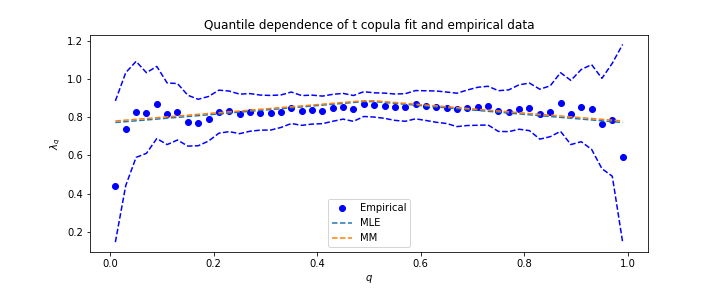
\includegraphics[width=\textwidth]{_pics/t Copula quantile dependence.png}
%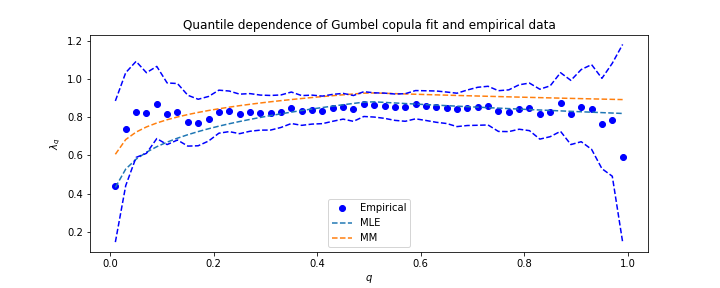
\includegraphics[width=\textwidth]{_pics/Gumbel Copula quantile dependence.png}
%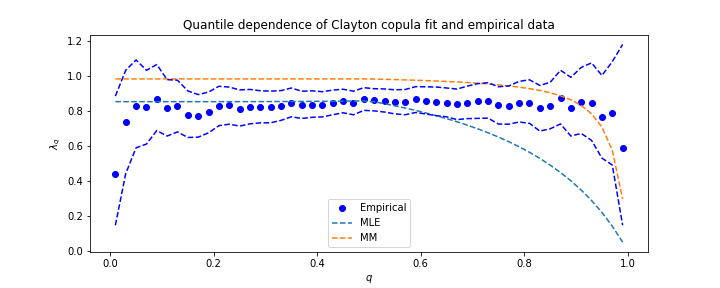
\includegraphics[width=\textwidth]{_pics/Clayton Copula quantile dependence.png}
%  \caption{}
%\label{fig:quantile dependence1}
%\end{figure}


The MM estimation perform just as we decided: match the upper and lower quantile dependence.




%
%
%\subsection{Two-Stage Estimation}\label{subsec:two-stage-estimation}
%~\cite{joe2005asymptotic} study the efficiency of a two-stage estimation procedure of copula estimation.
%The authors also call this method inference function for margins IFM.
%
%\textbf{Pros}
%\begin{enumerate}
%    \item Almost as efficient as MLE methods but easier to be implemented
%    \item Yields an asymptotically Gaussian, unbiased estimate
%\end{enumerate}
%
%\textbf{Cons}
%\begin{enumerate}
%    \item Subject to specification of marginals \cite{kim2007comparison}
%\end{enumerate}
%
%Our data
%\begin{align}
%    \pmb{y} = \begin{bmatrix}
%                  y_{11} & \cdots & y_{1i}\\
%                  \vdots & \ddots & \vdots \\
%                  y_{n1} & \cdots & y_{ni}
%                  \end{bmatrix}
%    \end{align}
%Let $F$ and $f$ be the joint cdf and joint density of $\pmb{y}$ with parameters $\pmb{\delta}$,
%and let $F_i$ and $f_i$ be the marginal cdf and marginal density for the $i^\text{th}$ random variable with parameters $\pmb{\theta}_i$, we have
%\begin{align}
%    f(\pmb{y}; \pmb{\theta}_1, \pmb{\theta}_2,\dots \pmb{\theta}_i, \pmb{\delta}) =
%    c\{F_1(\pmb{y}_1;\pmb{\theta}_1), F_2(\pmb{y}_2; \pmb{\theta}_2), \dots, F_i(\pmb{y}_1;\pmb{\theta}_i); \pmb{\delta}\}
%    \prod^i_{j=1}f_i(\pmb{y}_j;\pmb{\theta}_j)
%    \end{align}
%
%For a sample of size $n$, the log-likelihood of functions of the $i^\text{th}$ univariate margin is
%\begin{align}
%    L_i(\theta_i) = \sum^n_{m=1} \log f_i(y_{mi}; \theta_i),
%    \end{align}
%
%and the log-likelihood function for the joint distribution is
%\begin{align}
%    L(\delta, \theta_1, \theta_2, \dots, \theta_i) = \sum^n_{m=1}\sum^i_{j=1} \log f(y_{mj}; \delta, \theta_1, \theta_2, ..., \theta_i)
%    \end{align}
%
%In most cases, one does not have closed form estimators and numerical techniques are needed.
%Numerical ML estimation difficulty increase when the total number of parameters increases.
%The two-stage estimation is designed to overcome this problem.
%
%The two-stage procedure is
%\begin{enumerate}
%    \item estimate the univariate parameters from separate univariate likelihoods to get $\tilde{\pmb{\theta}_1}, ..., \tilde{\pmb{\theta}_i}$
%    \item maximize $L(\pmb{\delta}, \tilde{\pmb{\theta}_1}, \dots, \tilde{\pmb{\theta}_i})$ over $\pmb{\delta}$ to get $\tilde{\pmb{\delta}}$
%    \end{enumerate}
%
%Under regularity conditions
%\footnote{Regularity conditions include
%1. $\exists \frac{\partial \log f(x;\theta)}{\partial \theta}, \frac{\partial^2 \log f(x;\theta)}{\partial \theta^2}, \frac{\partial^3 \log f(x;\theta)}{\partial \theta^3}$ for all $x$;
%2. $\exists g(x), h(x) and H(x)$ such that for $\theta$ in a neighborhood $N(\theta_0)$ the relations
%$\left|\frac{\partial f(x;\theta)}{\partial theta}\right| \leq g(x)$,
%$\left|\frac{\partial^2 f(x;\theta)}{\partial \theta^2}\right| \leq h(x)$,
%$\left|\frac{\partial^3 f(x;\theta)}{\partial \theta^3}\right| \leq H(x)$ hold for all $x$, and
%$\int g(x) dx < \infty$, $\int h(x) dx < \infty$, $\mathbb{E}_\theta \{H(X)\} < \infty$ for $\theta \in N(\theta_0)$;
%3. For each $\theta \in \Theta$, $0< \mathbb{E}_\theta \left\{
%\left(
%\frac{\partial \log f(X;\theta)}{\partial \theta}
%\right)^2
%\right\}$. For detail see section 4.2.2 of~\cite{serfling2009approximation}}
%, $(\pmb{\tilde{\theta}}_1,\dots \pmb{\tilde{\theta}}_i, \pmb{\tilde{\delta}})$ is the solution of
%\begin{align}
%    (\partial L_1 / \partial \pmb{\theta}^\intercal_1,
%    \dots, \partial L_i / \partial \pmb{\theta}^\intercal_i, \partial L / \partial \pmb{\pmb{\delta}}^\intercal_1) = \pmb{0}
%    \end{align}
%
%For comparison, if we optimize $L$ directly without the two-stage procedure (i.e.~MLE), we solve for
%\begin{align}
%    (\partial L / \partial \pmb{\theta}^\intercal_1,
%    \dots, \partial L / \partial \pmb{\theta}^\intercal_i, \partial L / \partial \pmb{\pmb{\delta}}^\intercal_1) = \pmb{0}
%    \end{align}
%
%We denote the two solutions as
%$\tilde{\pmb{\eta}} = (\pmb{\tilde{\theta}}_1,\dots \pmb{\tilde{\theta}}_i, \pmb{\tilde{\delta}})$ for two-stage procedure;
%$\hat{\pmb{\eta}} =(\pmb{\hat{\theta}}_1,\dots \pmb{\hat{\theta}}_i, \pmb{\hat{\delta}})$ for MLE procedure.
%and compare the asymptotic relative efficiency of $\tilde{\pmb{\eta}}$ and $\hat{\pmb{\eta}}$.
%
%Asymptotics: yet to be done.\\
%~\cite{kim2007comparison} show the estimation of $\pmb{\theta}$ may be seriously affected.
%They compare the two-stage approach and Canonical Maximum Likelihood Method by simulation and
%conclude that Canonical Maximum Likelihood is prefered from a computational statistics and data analysis point of view.
%
%\subsection{Canonical Maximum Likelihood Method}\label{subsec:canonical-maximum-likelihood-method}
%This approach was studied by~\cite{genest1995semiparametric} and~\cite{shih1995inferences}.
%One estimates the margins using empirical CDF
%\begin{align}F_X(x)=\frac{1}{n+1}\sum_{i=1}^n 1(X_i \leq x)\end{align},
%
%we maximize the log-likelihood
%\begin{align}
%    L(\delta) = \sum_{i=1}^n \log [c_\delta \{F_X(X_i), F_Y(Y_i)\}]
%    \end{align}
%
%This procedure does not require specification of marginals.
%
%
%
%
%
%%also by Wang and Ding, 2000; Tsukahara, 2005
%%This is also known as pseudo maximum likelihood (PML) and as canonical maximum likelihood (see Cherubini et al., 2004)
%%
%%Genest and Werker (2002) obtained conditions under which the PMLE is asymptotically efficient.
%%
%%


\section{Data and margins}\label{sec:data-and-margins}
TODO:
\begin{itemize}
    \item Data description
    \item KDE and bandwidth selection
    \item plots
    \item Data preprocessing, the 300-30 train-test split, moving window estimation etc
\end{itemize}

\section{Results}
We illustrate the results in three directions, hedging effectiveness,
ability of hedging extreme negative events in $R^S$, and the stability of $h^*$.

\begin{itemize}
   \item  Hedging Effectiveness
   \begin{itemize}
     \item Kick out Frank for its ineffectiveness; Alternative to a one-parameter symmetric Archimedean copula is Plackett;
     \item Differences among combinations of copula and risk reduction objective are small;
     \item None of the combination can escape from the structural break point (dependence of training is stronger then that of testing). (The bump in 25-26th Sept 2019)
     \item The best performing RRO of a particular risk measure in out-of-sample $R^h$ is not necessarily same, e.g.
      VaR 95\% as RRO (with Gumbel copula) can generate the lowest out-of-sample ES 99\%.
   \end{itemize}
   \item Ability to hedge extreme events in $R^S$
   \begin{itemize}
     \item The extreme events in $R^S$ are well managed by the hedge.
     The magnitudes of loss in $R^h$ is much smaller than that of $R^h$. (Visually seen from the time series of $R^h$)
     \item None of the combination can escape from the structural break point (dependence of training is stronger then that of testing)
   \end{itemize}
   \item Stability of $h^\ast$
   \begin{itemize}
     \item Gumbel gives high $h$ all the time; the extreme events are "hedged" ex-ante.
     \item ES 99\% and VaR 99\% as risk reduction objective are too sensitive to extremes in training data;
     Large changes in $h$ are suggested in response to extremes training data, while the testing data are less extreme;
     \item ERM can be seen as a smoothed risk measure focusing in the lower tail of $R^h$; Less sensitive to rare events; Suggested.
   \end{itemize}
\item \end{itemize}


\subsection{Hedging Effectiveness}\label{subsec:hedging-effectiveness}
The hedging effectiveness(HE) is defined as
\begin{align}
  1- \frac{\rho_\phi(R^h)}{\rho_\phi(R^S)}.
  \end{align}
The hedging effectiveness is the reduction of portfolio risk.
This way of evaluating of hedging performance is proposed by \cite{ederington1979hedging} in the context of, at that time, hedging the newly introduced
organized futures market.
He evaluates the extent of variance reduction by introducing another asset.
We measure the hedging effectiveness also in other risk measure mentioned in section \ref{subsec:spectral-risk-measures},
for example
\begin{align}
  1- \frac{\text{ES}_\alpha(R^h)}{\text{ES}_\alpha(R^S)}.
  \end{align}

The box-plots in figure \ref{fig:OOSHE} show the out-of-sample hedging effectiveness of different copulas under various risk
reduction objectives across testing datasets.
Observe that in most of the copulas perform well in most of the time.
The average HE of copulas and risk reduction objectives is higher than 60\% except for Frank-copula.
However, the HEs vary a lot in different testing data.
In some instances, the HE can be as low as 10\%.
This reflects the highly violate nature of cryptocurrencies:
the optimal hedge ratio in the training data deviates from that of testing data.
There is a large literature about structural break points and time changing dependence, to name a few
\citet{hafner2012dynamic}, \citet{patton2006modelling}, \citet{creal2008general},
\citet{engle2002dynamic}, and \citet{giacomini2009inhomogeneous}.
\citet{manner2012survey} gives a great survey about this issue.
The discussion is out of the scope of this study.\medskip

Frank-copula, in general, is not a good choice to model financial data.
Figure~\ref{fig:Frank}

\begin{figure}[th]
   \centering
   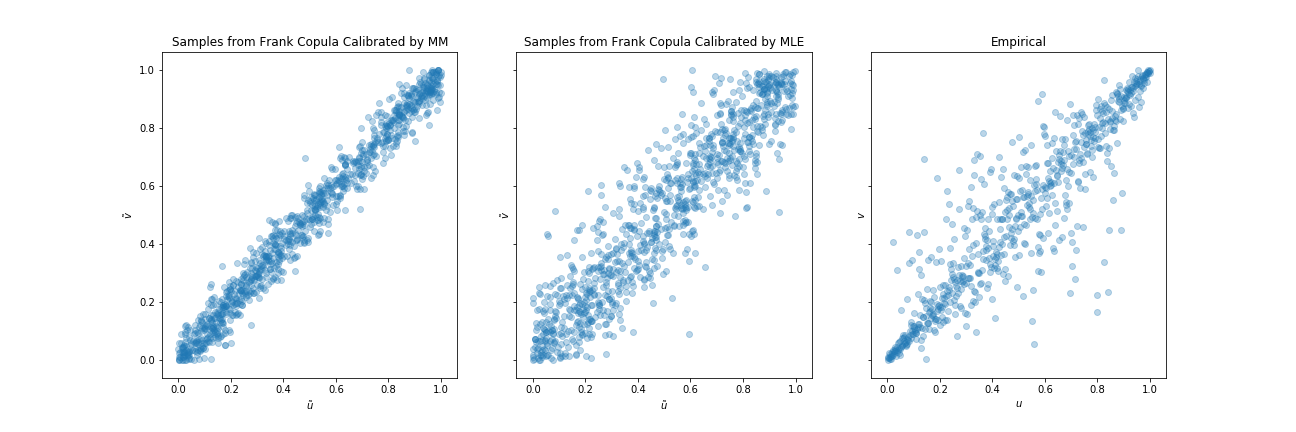
\includegraphics[width=\textwidth]{_pics/Frank.png}
   \caption{Comparison of Frank Copula Samples and Pseudo Observations of Bitcoin and CME Future Returns.
   }
   \label{fig:Frank}
\end{figure}

Aside from the Frank-copula, the HEs of various combination of copula and risk reduction objective are very similar.
This is an expected result as the portfolio consists only two assets.
In addition to hedging effectiveness, we observe the out-of-sample returns of the hedged portfolio.
Figure~\ref{fig:OOSRH} tabulates the time series of out-of-sample returns of hedged portfolio under various copulas and risk reduction objectives.

One can see all the combinations of copula and risk reduction objective generate a large fluctuation of returns in
25/09/2019 and 26/09/2019.
This large fluctuation is due to dependence break.
\medskip

\begin{figure}[th]
   \centering
   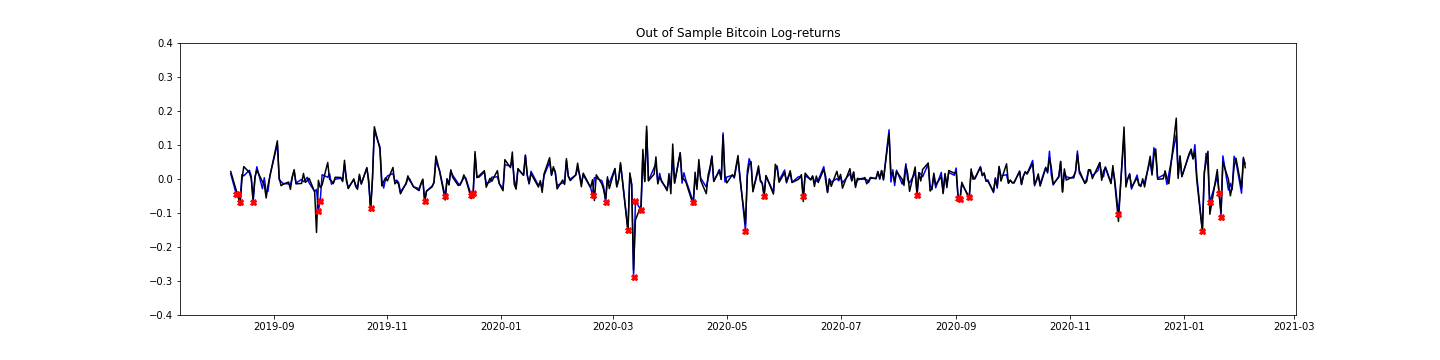
\includegraphics[width=\textwidth]{_pics/OOSBitcoin.png}
   \caption{Out of Sample Log-return of Bitcoin.
%   Lower Panel: Out of Sample Hedged Portfolio log-returns.
%   The $h^*$ is obtained from Gumbel copula aiming at reducing variance.
%   The red dots indicate the 30 most extreme negative returns in Bitcoin.
   }
   \label{fig:Gumbel}
\end{figure}

\newpage
\begin{landscape}
\begin{figure}[th]
   \centering
   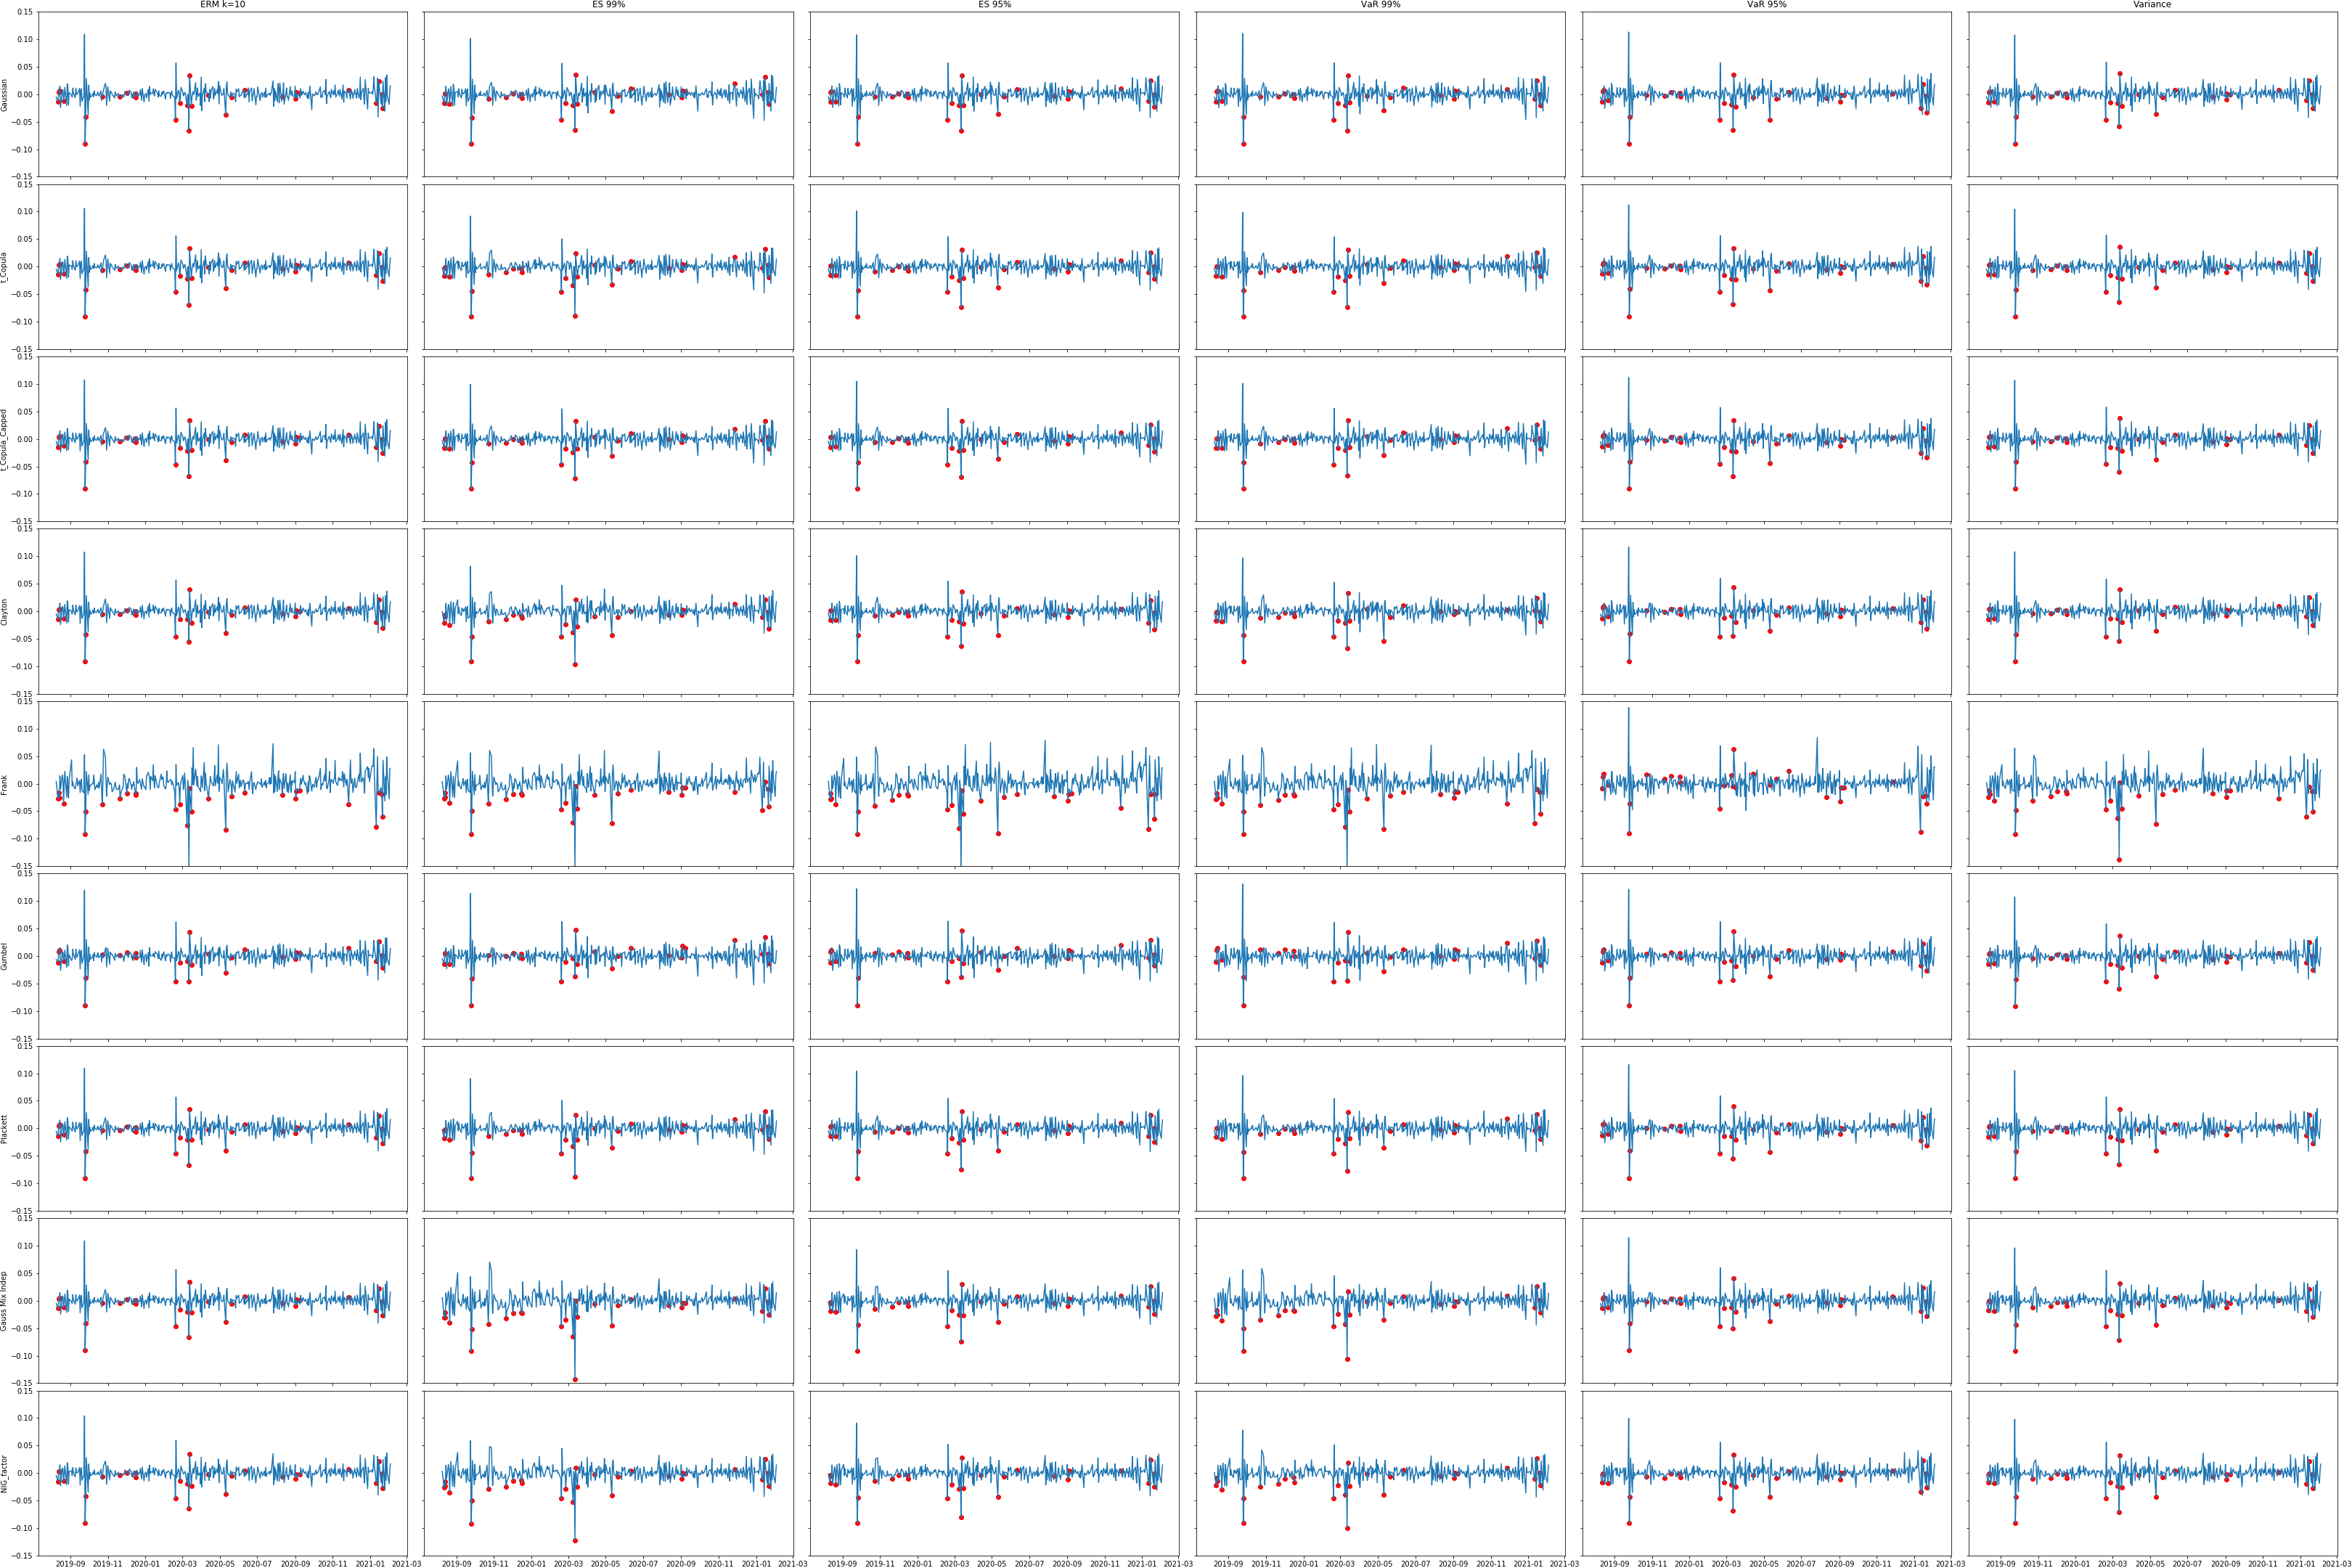
\includegraphics[width=\linewidth]{_pics/Rhs.png}
   \caption{Out-of-Sample Returns of Hedged Portfolio of Copulas and Risk Reduction Objectives.
   }
   \label{fig:OOSRH}
\end{figure}
\end{landscape}
\newpage

\newpage
\begin{landscape}
\begin{figure}[th]
   \centering
   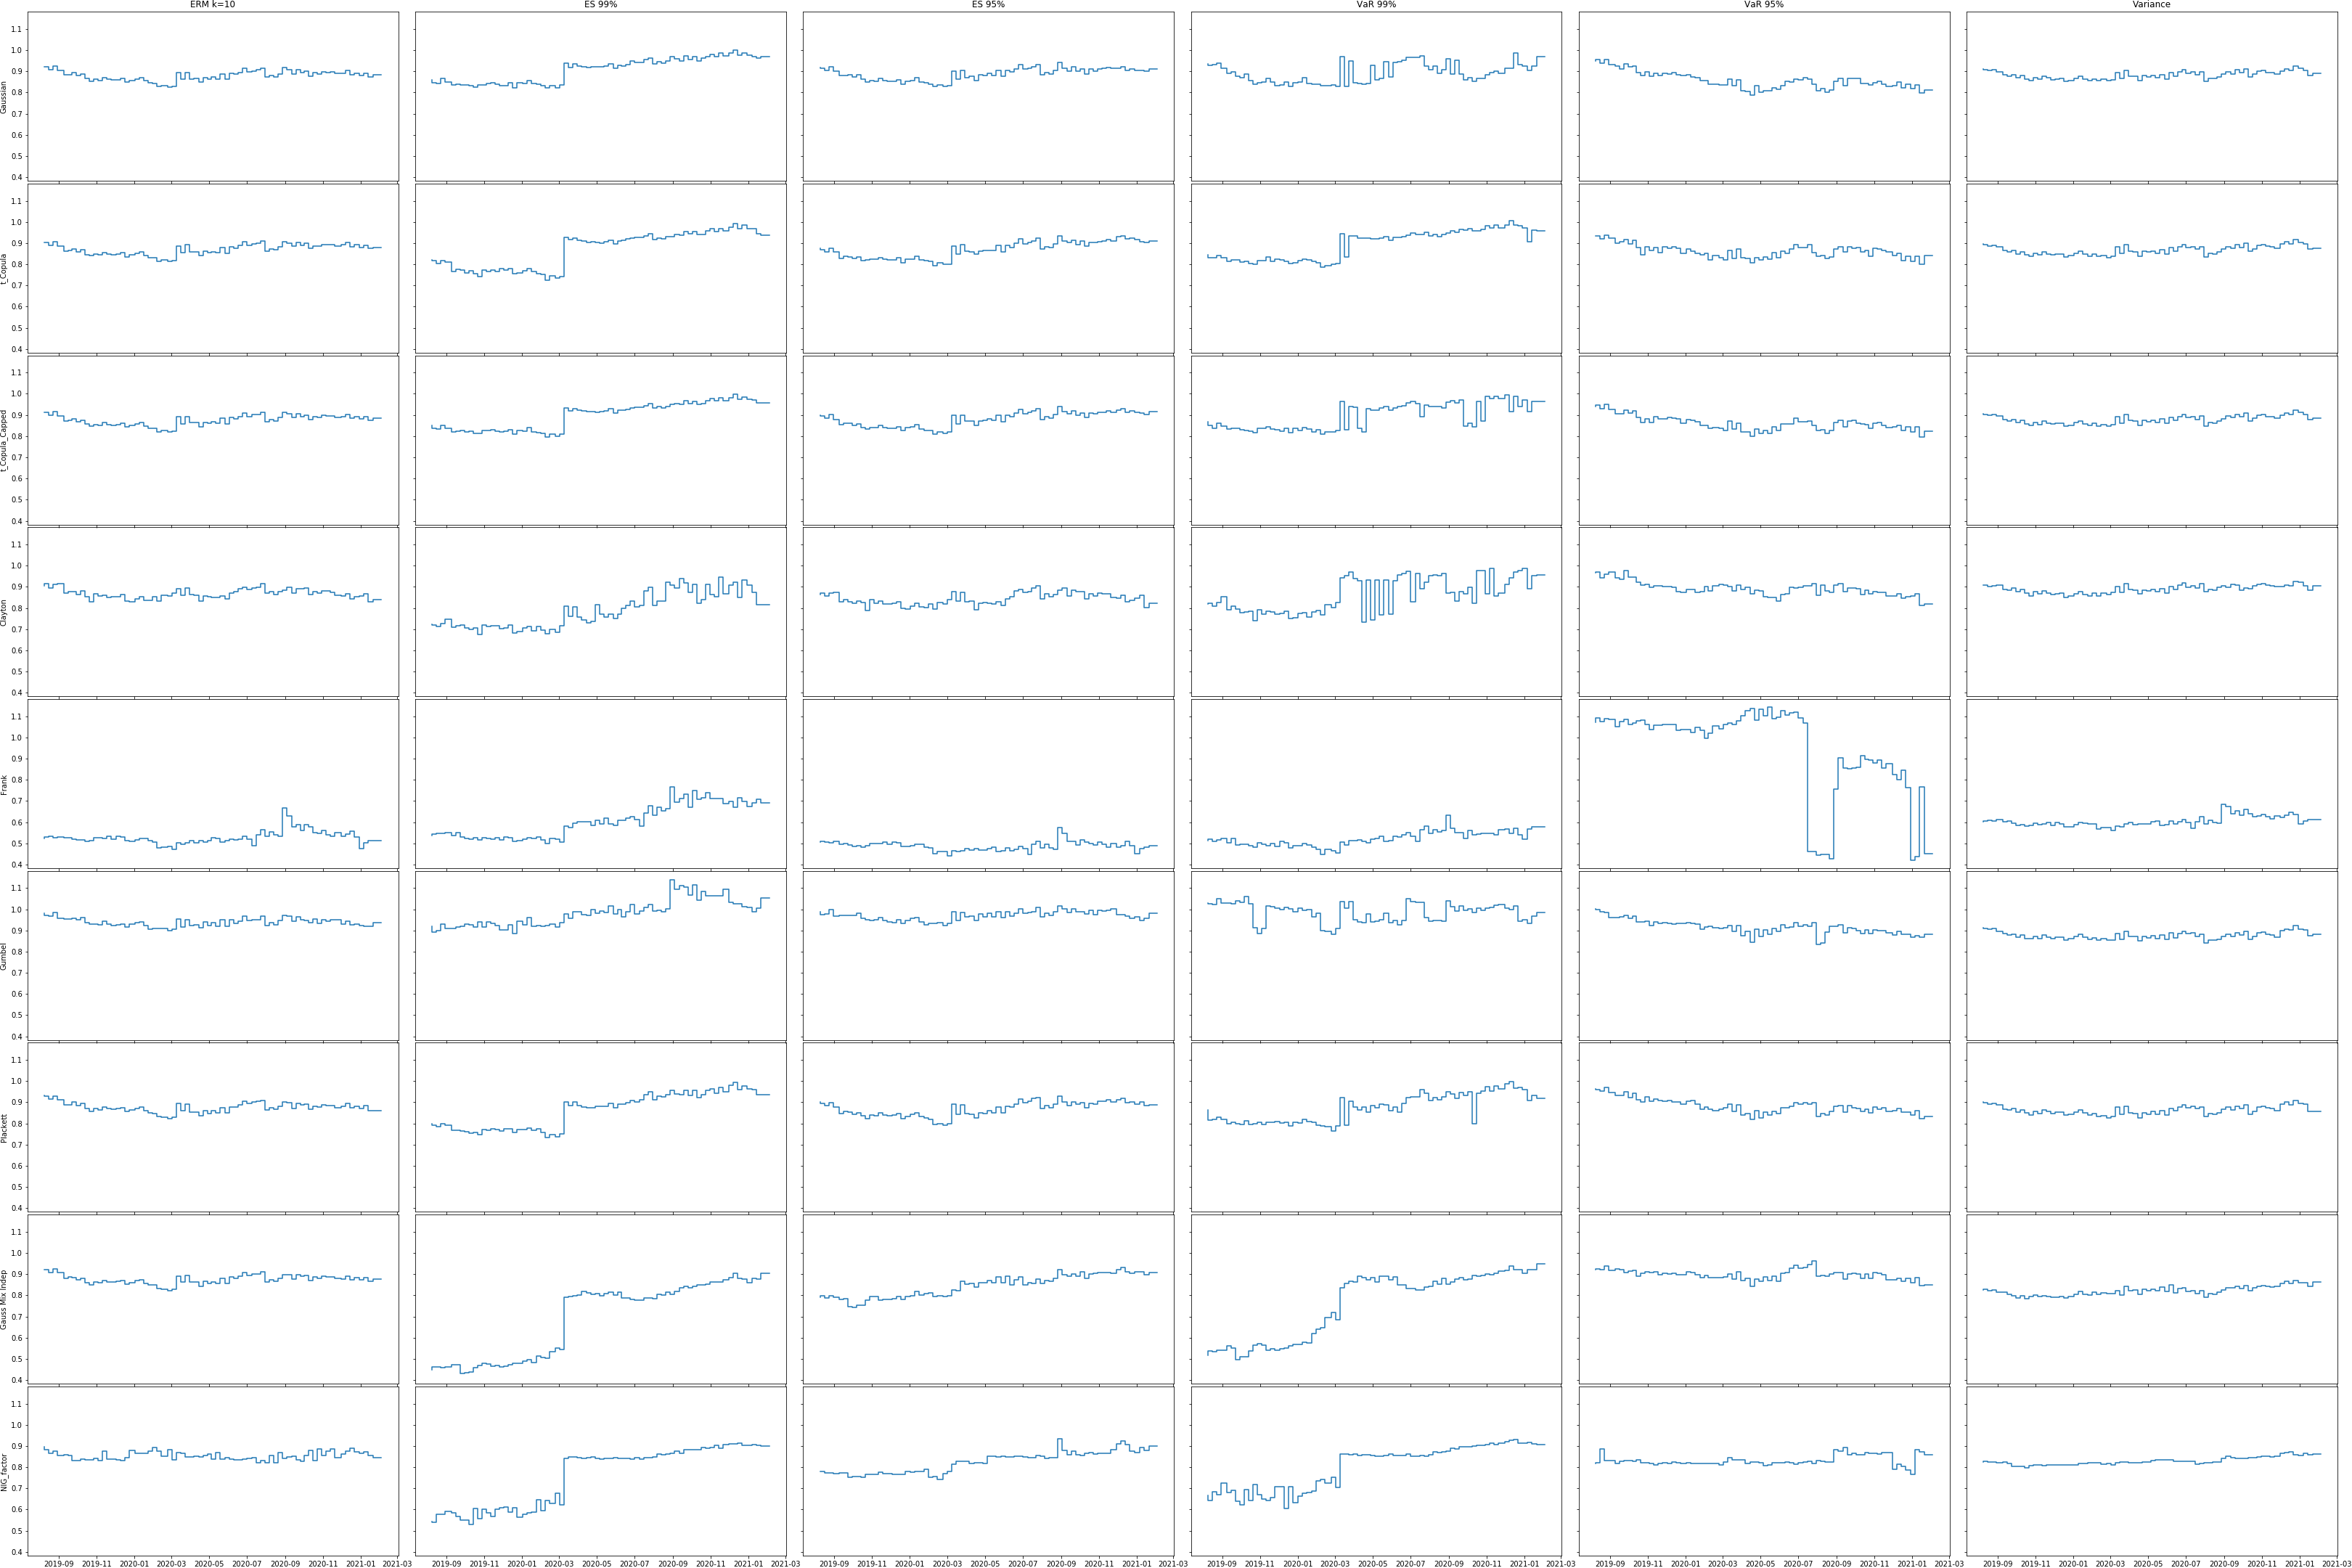
\includegraphics[width=\linewidth]{_pics/OHRs.png}
   \caption{Optimal Hedge Ratio Obtained from Combinations of Copula and Risk Reduction Objective.
   }
   \label{fig:OHRs}
\end{figure}
\end{landscape}
\newpage


%\begin{figure}[t]
%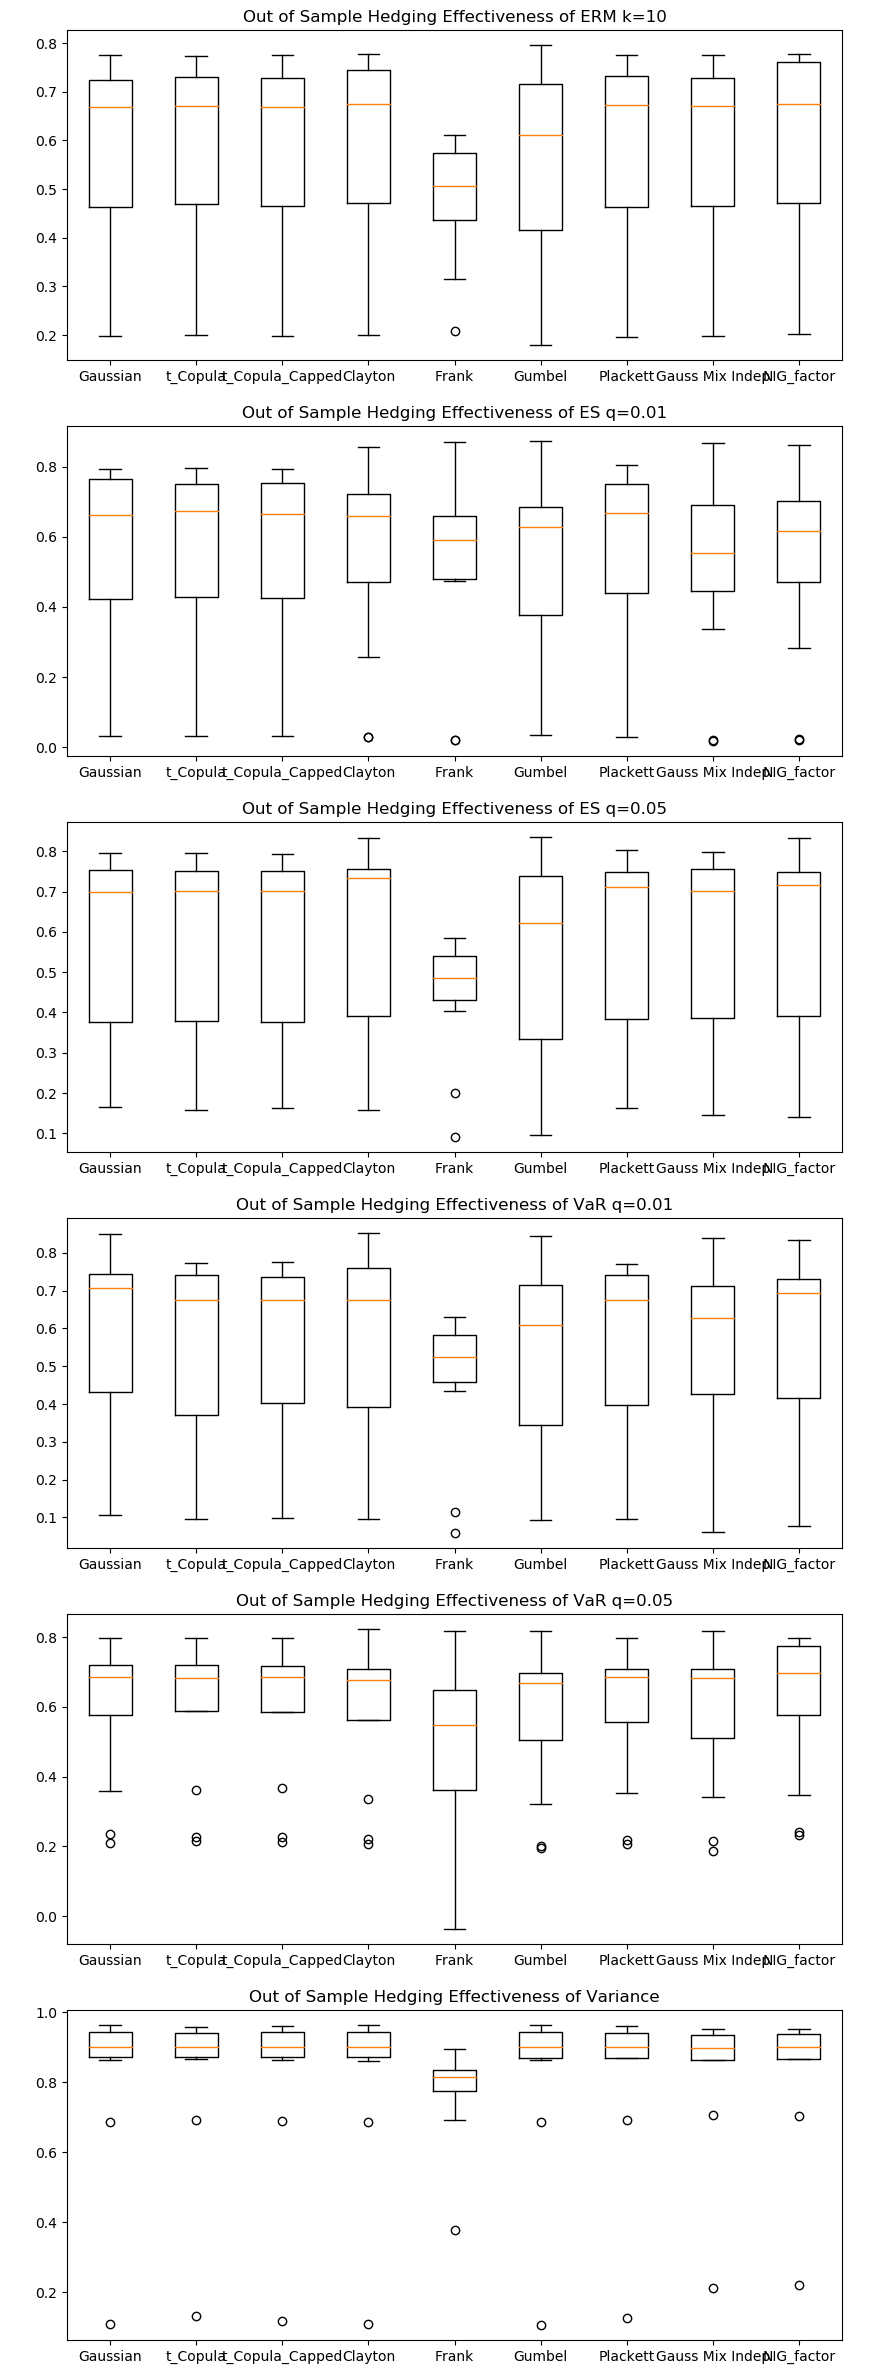
\includegraphics[width=\textwidth, height=\textheight]{_pics/Out of Sample Hedging Effectiveness.png}
%  \caption{}
%\label{out of Sample Hedging Effectieness}
%\end{figure}

\begin{figure}[!th]
   \centering
   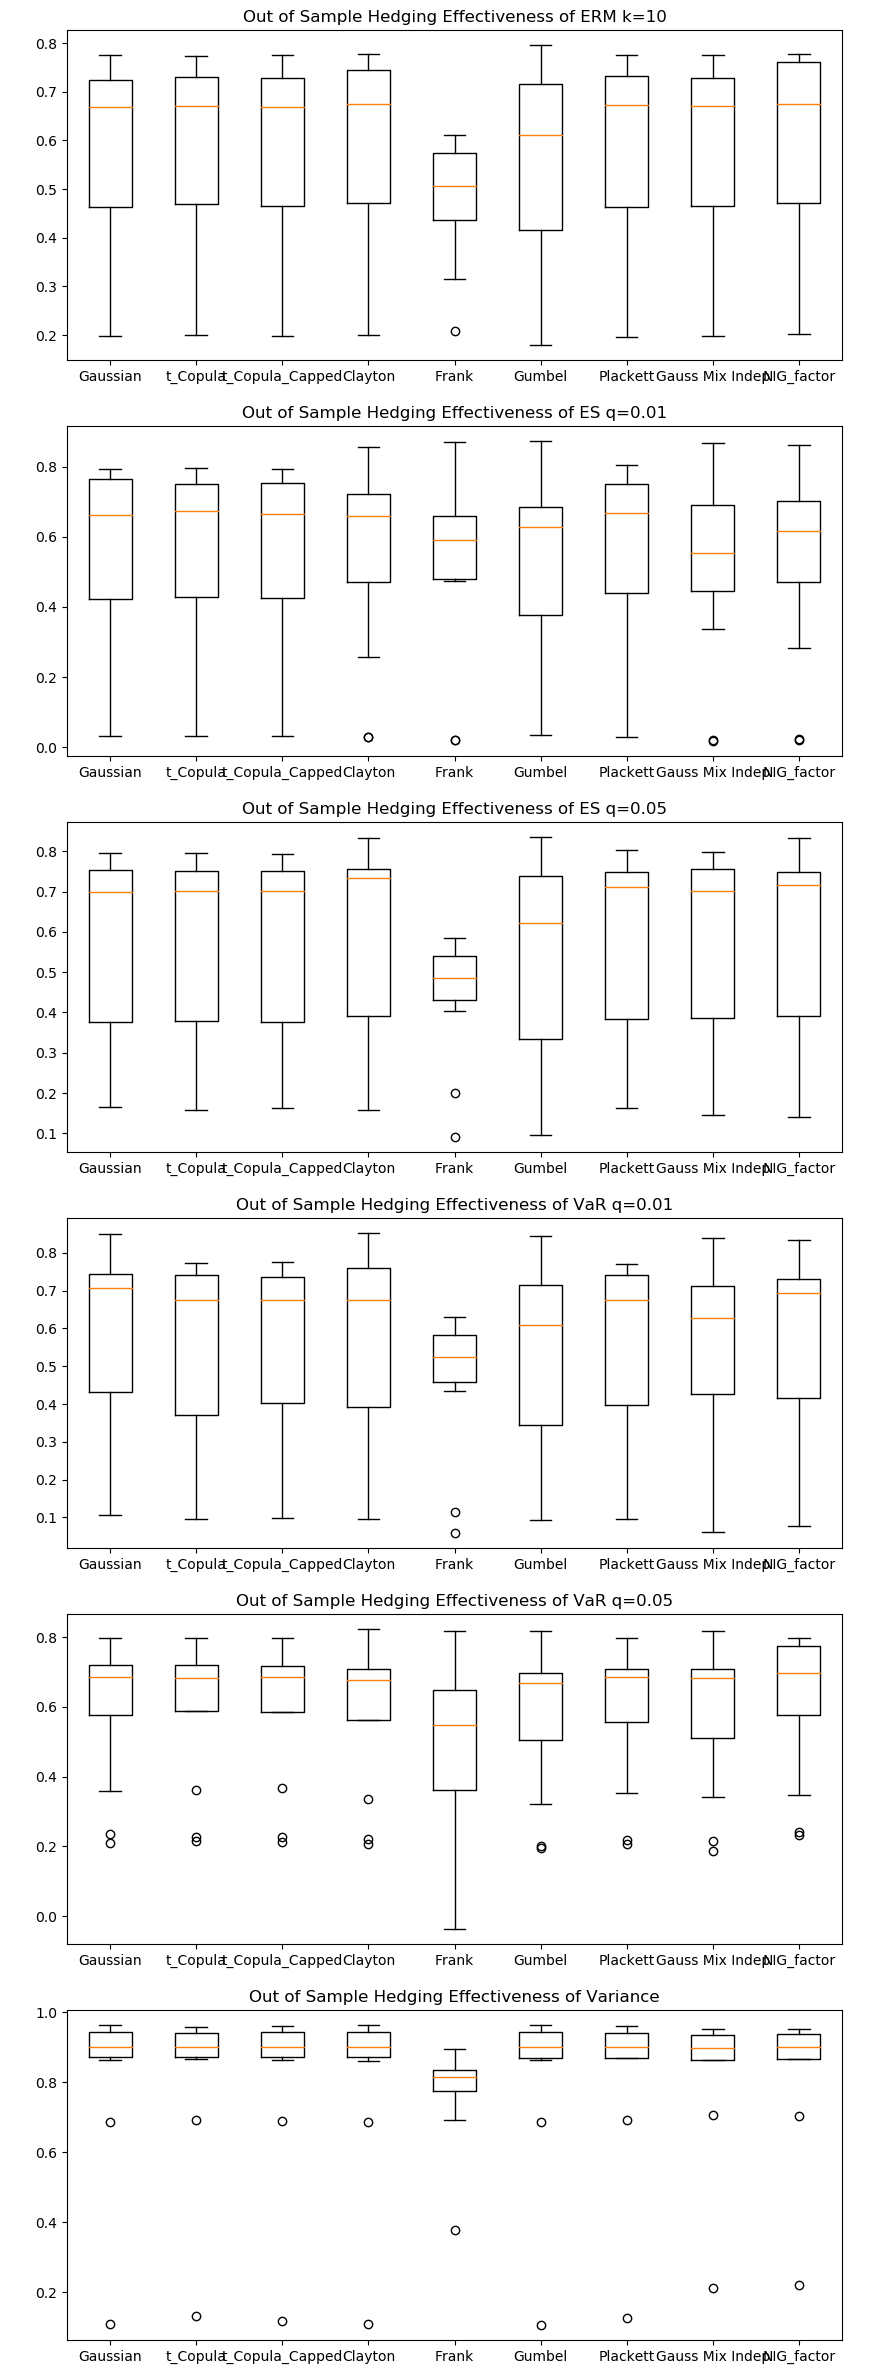
\includegraphics[height=25cm]{_pics/Out of Sample Hedging Effectiveness.png}
   \caption{Out of Sample Hedging Effectiveness Box-plot.
   The HEs are obtained from a set of out-of-sample data,
   each set consists 30 days log returns of Bitcoin and CME future.
   }
   \label{fig:OOSHE}
\end{figure}

Figure~\ref{fig:Gumbel} shows the time series of out-of-sample $R^h$ using Gumbel copula with the
objective of reducing variance.
The red dots are the 30 most extreme negative returns in Bitcoin.
In the figure, we can see the downside risk of Bitcoin is well managed by the hedging procedure with Gumbel copula.
Most of the extreme losses of Bitcoin are greatly reduced by introducing the CME future in the hedged portfolio.
Two exceptions are found in 25/09/2019 and 26/09/2019, where the CME future failed to follow the large drop in Bitcoin. (TODO: drop reason)
One of the possible reason is that traders was performing rollover activities on 25-26/09/2019, which
27/09/2019 is the expiry day of the September future.
Another reason for Gumbel fail of capturing the loss is dependence break.
The Kendall's tau in the training data is 0.2 higher than that of the testing data.
Other copulas suffer from the break as well.



\subsection{Stability of $h^*$}
We measure the stability of $h^*$ by sum of absolute change
\begin{align}
    \sum_{t=1}^T|h_t - h_{t-1}|.
    \end{align}

Adjustment of portfolio weights induces price slippage (ref) and transaction cost.
From figure \ref{SAD} we know the NIG factor copula with variance as risk reduction objective generates the smallest
sum of absolute change in OHR.

\begin{figure}[!th]
   \centering
   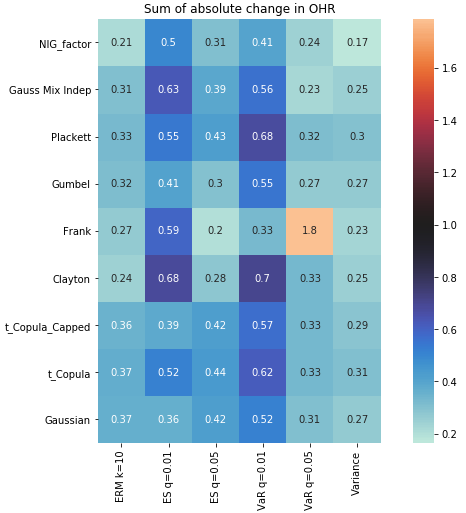
\includegraphics[width=\textwidth]{_pics/Sum of absolute change in OHR.png}
   \caption{Sum of Absolute Change in OHR.
   }
   \label{fig:SAD}
\end{figure}

%\usepackage{fontspec}
%\newcommand{\smallest}[1]{\textcolor{Maroon}{\textbf{#1}}}

\begin{table}
\begin{tabular}{lrrrrrr}
\toprule
{} &  ERM k=10 &    ES 99\% &    ES 95\% &   VaR 99\% &   VaR 95\% &  Variance \\
\midrule
Gaussian        &  0.019985 &  0.020802 &  0.020061 &  0.020230 &  0.019983 &  \color{blue}0.019757 \\
t\_Copula        &  0.020097 &  0.021698 &  0.020381 &  0.020966 &  0.020071 &  \color{blue}0.019890 \\
t\_Copula\_Capped &  0.020048 &  0.021018 &  0.020202 &  0.020554 &  0.020059 &  \color{blue}0.019792 \\
Clayton         &  0.019519 &  0.021341 &  0.019789 &  0.021045 &  \color{blue}0.019389 &  0.019675 \\
Frank           &  0.029234 &  0.026240 &  0.030770 &  0.029157 &  \color{blue}0.023085 &  0.025928 \\
Gumbel          &  0.020014 &  0.021411 &  0.020511 &  0.021643 &  \color{blue}0.019557 &  0.019757 \\
Plackett        &  0.020010 &  0.021531 &  0.020363 &  0.020870 &  \color{blue}0.019755 &  0.019909 \\
Gauss Mix Indep &  0.019949 &  0.025390 &  0.020454 &  0.023283 &  \color{blue}0.019667 &  0.020006 \\
NIG\_factor      &  \color{blue}0.019720 &  0.023425 &  0.020706 &  0.022039 &  0.019950 &  0.019999 \\
\bottomrule
\end{tabular}
\caption{Exponential Risk Measure $k=10$}
\end{table}

\begin{table}
\begin{tabular}{lrrrrrr}
\toprule
{} &  ERM k=10 &    ES 99\% &    ES 95\% &   VaR 99\% &   VaR 95\% &  Variance \\
\midrule
Gaussian        &  0.061084 &  0.062405 &  0.061201 &  0.062148 &  0.061712 &  \color{blue}0.059310 \\
t\_Copula        &  0.062148 &  0.068702 &  0.063339 &  0.063964 &  0.062067 & \color{blue}0.060735 \\
t\_Copula\_Capped &  0.061623 &  0.064114 &  0.062198 &  0.062466 &  0.062072 & \color{blue}0.059676 \\
Clayton         &  0.058495 &  0.069910 &  0.060812 &  0.064595 &  \color{blue}0.055962 &  0.058318 \\
Frank           &  0.104185 &  0.096795 &  0.108713 &  0.105070 &  \color{blue}0.068457 &  0.091321 \\
Gumbel          &  0.056513 &  0.059574 &  0.056035 &  0.058162 &  \color{blue}0.055492 &  0.059525 \\
Plackett        &  0.061167 &  0.068027 &  0.063426 &  0.064563 &  \color{blue}0.058491 &  0.061017 \\
Gauss Mix Indep &  0.061157 &  0.088023 &  0.063900 &  0.073316 &  \color{blue}0.057007 &  0.063081 \\
NIG\_factor      &  \color{blue}0.060878 &  0.078959 &  0.065270 &  0.070919 &  0.062097 &  0.062848 \\
\bottomrule
\end{tabular}
\caption{ES 99\%}
\end{table}

\begin{table}
\begin{tabular}{lrrrrrr}
\toprule
{} &  ERM k=10 &    ES 99\% &    ES 95\% &   VaR 99\% &   VaR 95\% &  Variance \\
\midrule
Gaussian        &  0.034488 &  0.035237 &  0.034548 &  0.035123 &  0.034838 &  \color{blue}0.034248 \\
t\_Copula        &  0.034777 &  0.037100 &  0.035234 &  0.035634 &  0.035055 &  \color{blue}0.034494 \\
t\_Copula\_Capped &  0.034647 &  0.035679 &  0.034862 &  0.035282 &  0.034937 &  \color{blue}0.034322 \\
Clayton         &  0.033714 &  0.037282 &  0.034230 &  0.036089 &  \color{blue}0.033445 &  0.034046 \\
Frank           &  0.053661 &  0.047849 &  0.056299 &  0.053409 &  \color{blue}0.037638 &  0.046953 \\
Gumbel          &  0.034028 &  0.035965 &  0.034528 &  0.036353 &  \color{blue}0.033568 &  0.034293 \\
Plackett        &  0.034592 &  0.036831 &  0.035316 &  0.035752 &  \color{blue}0.034186 &  0.034558 \\
Gauss Mix Indep &  0.034439 &  0.045160 &  0.035120 &  0.040027 &  \color{blue}0.033756 &  0.034478 \\
NIG\_factor      &  \color{blue}0.033882 &  0.041001 &  0.035677 &  0.037975 &  0.034656 &  0.034453 \\
\bottomrule
\end{tabular}
\caption{ES 95\%}
\end{table}

\begin{table}
\begin{tabular}{lrrrrrr}
\toprule
{} &  ERM k=10 &    ES 99\% &    ES 95\% &   VaR 99\% &   VaR 95\% &  Variance \\
\midrule
Gaussian        &  \color{blue}0.041327 &  0.044416 &  0.041943 &  0.043399 &  0.042275 &  0.041981 \\
t\_Copula        &  \color{blue}0.041450 &  0.044830 &  0.042806 &  0.043789 &  0.041693 &  0.041969 \\
t\_Copula\_Capped &  \color{blue}0.041498 &  0.044169 &  0.042411 &  0.044051 &  0.042018 &  0.042056 \\
Clayton         &  \color{blue}0.040022 &  0.044523 &  0.042878 &  0.044215 &  0.040913 &  0.041943 \\
Frank           &  0.076644 &  0.055387 &  0.081273 &  0.073433 &  \color{blue}0.046177 &  0.061056 \\
Gumbel          &  0.042079 &  0.042139 &  0.042187 &  0.045340 &  \color{blue}0.040523 &  0.041937 \\
Plackett        &  \color{blue}0.041013 &  0.044971 &  0.042370 &  0.042995 &  0.041574 &  0.041731 \\
Gauss Mix Indep &  0.040998 &  0.048017 &  0.043249 &  0.044518 &  \color{blue}0.040749 &  0.043386 \\
NIG\_factor      &  \color{blue}0.040457 &  0.047201 &  0.043925 &  0.044230 &  0.043240 &  0.043138 \\
\bottomrule
\end{tabular}
\caption{VaR 99\%}
\end{table}

\begin{table}
\begin{tabular}{lrrrrrr}
\toprule
{} &  ERM k=10 &    ES 99\% &    ES 95\% &   VaR 99\% &   VaR 95\% &  Variance \\
\midrule
Gaussian        &  0.020385 &  0.020315 &  0.020143 &  0.020412 &  0.020121 &  \color{blue}0.019579 \\
t\_Copula        &  0.020547 &  0.020428 &  0.020661 &  0.020611 &  0.020370 &  \color{blue}0.019820 \\
t\_Copula\_Capped &  0.020525 &  0.020544 &  0.020503 &  0.020486 &  0.020224 &  \color{blue}0.019656 \\
Clayton         &  0.019702 &  0.021042 &  0.020143 &  0.020640 &  0.019990 &  \color{blue}0.019700 \\
Frank           &  0.026372 &  0.023529 &  0.027105 &  0.026212 &  \color{blue}0.023389 &  0.023594 \\
Gumbel          &  0.019781 &  0.021311 &  0.020716 &  0.020421 &  \color{blue}0.019077 &  0.019541 \\
Plackett        &  0.020459 &  0.020257 &  0.020589 &  0.020100 &  0.020237 &  \color{blue}0.020047 \\
Gauss Mix Indep &  0.020482 &  0.024753 &  0.020304 &  0.024158 &  \color{blue}0.019944 &  0.020723 \\
NIG\_factor      &  \color{blue}0.019923 &  0.023784 &  0.021009 &  0.022172 &  0.019980 &  0.020670 \\
\bottomrule
\end{tabular}
\caption{VaR 95\%}
\end{table}

\begin{table}
\begin{tabular}{lrrrrrr}
\toprule
{} &  ERM k=10 &    ES 99\% &    ES 95\% &   VaR 99\% &   VaR 95\% &  Variance \\
\midrule
Gaussian        &  0.014387 &  0.014380 &  0.014360 &  0.014530 &  0.014670 &  \color{blue}0.014294 \\
t\_Copula        &  0.014378 &  0.014626 &  0.014343 &  0.014385 &  0.014627 &  \color{blue}0.014306 \\
t\_Copula\_Capped &  0.014375 &  0.014418 &  0.014332 &  0.014430 &  0.014643 &  \color{blue}0.014290 \\
Clayton         &  0.014306 &  0.014870 &  0.014332 &  0.014532 &  0.014493 &  \color{blue}0.014267 \\
Frank           &  0.021495 &  0.018982 &  0.022736 &  0.021476 &  \color{blue}0.018142 &  0.018897 \\
Gumbel          &  0.014618 &  0.014971 &  0.014878 &  0.015438 &  0.014622 &  \color{blue}0.014321 \\
Plackett        &  0.014444 &  0.014560 &  0.014424 &  0.014423 &  0.014596 &  \color{blue}0.014353 \\
Gauss Mix Indep &  0.014404 &  0.017404 &  \color{blue}0.014341 &  0.015671 &  0.014453 &  0.014408 \\
NIG\_factor      &  \color{blue}0.014362 &  0.015841 &  0.014484 &  0.015043 &  0.014474 &  0.014415 \\
\bottomrule
\end{tabular}
\caption{Standard Deviation}
\end{table}

\newpage
\bibliographystyle{abbrvnamed} %
\bibliography{finance} %
\newpage
\section{Appendix}\label{sec:appendix}

\begin{proposition}
   Let $\bm{X} = (X_1, ..., X_d)^\top$ be real-valued random variables with corresponding
   copula density $\bm{c}_{X_1, ..., X_d}$, and continuous marginals $F_{X_1}, ..., F_{X_d}$.
   Then,
   density of the linear combination of marginals $Z = n_1 \cdot X_1 + ... +  n_d \cdot X_d $ is

   \begin{align}
   f_Z(z) &= \left| n_1^{-1} \right| \int_{[0,1]^{d-1}} \left[ \bm{c}_{X_1,...,X_d}
      \{F_{X_1} \circ S(z), u_2, ..., u_d \} \cdot
      f_{X_1} \circ S(z) \right] du_2 ... du_d \label{density} \\
      S(z) &= \frac{1}{n_1}\cdot z - \frac{n_2}{n_1} \cdot F^{-1}_{X_2}(u_2) - ... -  \frac{n_d}{n_1} \cdot F^{-1}_{X_d}(u_d)
      \end{align}
   \end{proposition}

\begin{proof} \medskip
   Rewrite $Z = n_1 \cdot X_1 + ... +  n_d \cdot X_d $ in matrix form
   \begin{align}
      \begin{bmatrix}
      Y \\ X_2 \\ \vdots \\ X_d
      \end{bmatrix}
      = \begin{bmatrix}
      n_1    & n_2   & \cdots & n_d     \\
      0      & 1     &  \cdots & 0       \\
      \vdots &       & \ddots & \vdots \\
      0      & \cdots &       & 1  \\
      \end{bmatrix}
      \begin{bmatrix}
         X_1 \\ X_2 \\ \vdots \\ X_d
      \end{bmatrix}
      = \bm{A}
      \begin{bmatrix}
         X_1 \\ X_2 \\ \vdots \\ X_d
      \end{bmatrix}.
      \end{align} \medskip

   By transformation variables
   \begin{align}
      \bm{f}_{Z,X_2,...,X_d}(z, x_2, ...,x_d) &= \bm{f}_{X_1,...,X_d}\left( \bm{A}^{-1}
      \begin{bmatrix}
         z \\ x_2 \\ \vdots \\ x_d
      \end{bmatrix}
      \right)  \cdot |\det \bm{A}^{-1}| \\
      &= \left| n_1^{-1} \right| \bm{f}_{X_1,...,X_d}\{S(z), x_2,...,x_d\}
      \end{align} \medskip

   Let $u_i = F_{X_i}(x_i)$ and
   use the relationship
   \begin{align}
      \bm{c}_{X_1,...,X_d}(u_1, ..., u_d)=\frac{\bm{f}_{X_1,...,X_d}(x_1,...,x_d)}{\prod_{i=1}^d f_{X_i}(x_i)},
   \end{align}
   we have
   \begin{align}
     & \bm{f}_{Z,X_2,...,X_d}(z, x_2, ...,x_d) = \\
      & \left| n_1^{-1} \right| \cdot
      \bm{c}_{X_1,...,X_d}\{F_{X_1} \circ S(z), u_2, ...,  u_d\}  \cdot
      f_{X_1} \{ S(z) \} \cdot
      \prod_{i=2}^d f_{X_i}(x_i)
      \end{align}

   The claim \ref{density} is obtained by integrating out $x_2, ... x_d$ by substituting $dx_i = \frac{1}{f_{X_i}(x_i)}du_i$.
   \end{proof}
\end{document}
